\documentclass[journal]{IEEEtran}

% IEEE Access uses the standard IEEEtran journal class.
\usepackage[T1]{fontenc}
% Map literal Unicode em-dashes to the LaTeX `---` ligature so the source compiles
% identically under pdflatex and the XeTeX engine used by `make pdf` (tectonic).
\usepackage{newunicodechar}
\newunicodechar{—}{---}
\usepackage{amsmath}
\usepackage{amsfonts}
\usepackage{booktabs}
\usepackage{array}
\usepackage{multirow}
\usepackage{xcolor}
\usepackage{graphicx}
\usepackage{subcaption}
\usepackage{listings}
\usepackage{tikz}
\usetikzlibrary{arrows.meta, positioning, shapes.geometric, fit, backgrounds}
\usepackage{pgfplots}
\pgfplotsset{compat=1.18}
\usepackage{url}
\usepackage[hidelinks]{hyperref}

% YAML is not a built-in listings language — define a minimal dialect.
\lstdefinelanguage{yaml}{
  keywords={true,false,null},
  sensitive=true,
  comment=[l]{\#},
  morestring=[b]",
  morestring=[b]',
}

% Code listing style
\lstset{
  basicstyle=\ttfamily\footnotesize,
  breaklines=true,
  frame=single,
  backgroundcolor=\color{gray!8},
}

% -----------------------------------------------------------------------
\title{VisionServe: A Lean, License-Safe Inference Server for Computer Vision}

\author{Trung~Minh~Bui%
  \thanks{T. M. Bui is with the Korea Electronics Technology Institute (KETI),
  Seongnam, South Korea (e-mail: minhtrung@keti.re.kr).}}

\begin{document}
\maketitle

% -----------------------------------------------------------------------
\begin{abstract}
Open-source model hubs let a server load weights whose declared license cannot be trusted:
recent audits find that 95.8\% of models lack the required license text and that 35.5\% of
model-to-application transitions silently strip restrictive (copyleft)
clauses~\cite{jewitt2026permissivewashing,jewitt2025licensedrift}. For a permissively licensed
project, loading one AGPL model relicenses the whole
deployment~\cite{ultralytics2023yolo,agpllicense}. We present VisionServe, a single-binary Go
inference server whose primary contribution is a load-time license-policy gate. At model-load
time the gate refuses any model whose declared license is outside a permissive allowlist
(Apache-2.0, MIT, BSD), and in a verified mode it binds each declared license to specific weight
bytes (sha256), an audited source URL, and a maintainer-audited provenance ledger; a reproducible
adversarial test shows the gate rejecting relabeled, tampered, and unaudited models. To our
knowledge no prior inference runtime enforces a license policy at load time. Existing tools either
analyze and warn at build time or verify container identity at deploy time. The ledger separates
authority between contributors, who edit manifests, and maintainers, who audit upstreams, so a
relabeled manifest is rejected by a record its author does not control. The gate is a
policy-enforcement point, not a license oracle for arbitrary uploads.

Around this gate we build a complete Python-free computer-vision serving stack and measure it on
an NVIDIA RTX A6000 and a Jetson AGX Orin. On identical ONNX the single Go binary matches an
eight-process FastAPI+ONNX-Runtime deployment in peak goodput while using a fraction of the
memory; against the single-worker default that most teams ship it reaches roughly $8\times$ the
goodput. A latency decomposition attributes the per-request cost to pure-Go JPEG decode rather
than the GPU (ONNX-Runtime inference under 1\,ms), and with a pre-decoded tensor VisionServe
matches a default-configuration NVIDIA Triton's serving ceiling. Export and serving preserve
ImageNet Top-1 accuracy to within 0.5\%. VisionServe serves 19 registered models across seven task
types, including a pure-Go analytic planar-grasp synthesizer that needs no extra weights, and is
released under the Apache-2.0 license.

\end{abstract}

\begin{IEEEkeywords}
Computer vision, inference serving, model licensing, software supply chain, edge
computing, ONNX Runtime, open-vocabulary detection.
\end{IEEEkeywords}

% -----------------------------------------------------------------------
\IEEEpeerreviewmaketitle

\section{Introduction}
\label{sec:intro}
Computer vision models have moved rapidly from research prototypes into production pipelines
and edge deployments, powering applications from autonomous inspection robots to real-time
video analytics at the network edge.

\paragraph{Problem.}
General-purpose model-serving systems such as NVIDIA Triton Inference Server~\cite{nvidia2023triton}
and TorchServe~\cite{pytorch2023torchserve} are architected for cloud data centers: they
require Kubernetes or Docker orchestration, expose complex gRPC configuration surfaces, and
carry Python or JVM runtimes that can exceed several gigabytes of disk and memory overhead.
At the other extreme, deploying a model by running a bare PyTorch script provides neither
a stable REST API, nor lifecycle management (loading, unloading, VRAM accounting), nor the
ability to serve multiple models through a single endpoint.
Compounding the infrastructure problem is a license minefield: the most widely used
detection models---the YOLO series---are released under the GNU Affero General Public
License v3.0 (AGPL-3.0)~\cite{ultralytics2023yolo,agpllicense}, which requires any software
that incorporates or exposes YOLO as a network service to publish its entire source code
under AGPL-3.0, foreclosing use in closed-source or commercial products without a
paid commercial license.

\paragraph{Gap.}
Despite the wide variety of available tools, no existing solution simultaneously provides
(a)~a complete CV serving stack---covering detection, segmentation, open-vocabulary
detection, classification, depth estimation, and embedding---in a single deployable unit;
(b)~a guarantee that every included model is permissively licensed (Apache-2.0, MIT, or
BSD) so that downstream products can use it without license encumbrance; and
(c)~a single self-contained binary that runs on edge hardware without requiring a Python
interpreter, GPU driver stack beyond what ONNX Runtime needs, or container runtime.

\paragraph{VisionServe.}
We present VisionServe, a lightweight inference server written in Go that is designed to be
the ``Ollama for Computer Vision''~\cite{ollama2023}: one binary, pulled from a local model
registry, serving any of 16 registered models over a REST API with no Python dependency.
All inference is delegated to ONNX Runtime~\cite{onnxruntime} via a thin cgo binding,
enabling automatic fallback across execution providers (TensorRT $\to$ CUDA $\to$ CoreML
$\to$ DirectML $\to$ OpenVINO $\to$ CPU) without changes to model code.
License safety is enforced structurally: the model registry parser validates each model's
declared license against an Apache-2.0/MIT/BSD allowlist at server startup, refusing to
load any model that does not pass.

\paragraph{Contributions.}
This paper makes the following contributions:

\begin{itemize}
  \item \textbf{A license-enforcing model loader (primary).} To our knowledge the first
        inference runtime to enforce a permissive-license allowlist (Apache-2.0/MIT/BSD)
        \emph{at model-load time}, refusing non-permissive models by construction, and binding
        the declared license to specific weight bytes (sha256) and an audited
        \texttt{source\_url}, entirely offline in a single edge binary.

  \item \textbf{A novelty boundary and threat model.} We position the gate against build-time
        SCA scanners, deploy-time admission controllers, and model signing---none of which
        enforces a license policy at model-load time---and give an honest threat model
        exercised by a reproducible adversarial demo (an AGPL-declared model, a weight-hash
        mismatch, and an unaudited source are each refused).

  \item \textbf{A CV-specific serving-overhead crossover characterization (measured).} On
        identical ONNX, a single-binary Go server scales to $\sim$$8\times$ a GIL-bound
        FastAPI+ONNX~Runtime baseline's peak goodput (695 vs.\ 85~rps for MobileNetV3-Small at
        concurrency~64), and we report honestly where it loses ($\sim$78\,ms vs.\
        $\sim$15\,ms per request at concurrency~1).

  \item \textbf{A latency decomposition localizing the overhead} to pure-Go JPEG decode
        ($\sim$19\,ms) and resize/normalize ($\sim$3.6\,ms), not the GPU (ORT~Run $<$1\,ms on
        an A6000)---the CV-specific instance of non-inference overhead dominating small-DNN
        serving~\cite{abouelhamayed2024beyond}.

  \item \textbf{A reproducible end-to-end evaluation:} served accuracy (export and serving
        preserve ImageNet Top-1 to within 0.5\%), throughput--latency behavior across
        concurrency, and multi-model footprint (one Go process serving four models uses
        917\,MB RSS / 920\,MB VRAM vs.\ 1632\,MB / 1384\,MB for four FastAPI+ORT processes),
        plus a single unified result schema and Python/JavaScript client libraries across all
        16 registered models (12 benchmarked) on an NVIDIA RTX~A6000.
\end{itemize}

\paragraph{Paper outline.}
The remainder of this paper is organized as follows: Section~\ref{sec:related} surveys
related work in model serving and CV tooling; Section~\ref{sec:design} describes the
system architecture and key design decisions; Section~\ref{sec:catalog} presents the model
catalog; Section~\ref{sec:eval} reports benchmark results; Section~\ref{sec:applications}
illustrates representative use cases; and Sections~\ref{sec:limitations}
and~\ref{sec:conclusion} discuss limitations, future directions, and conclusions.


% -----------------------------------------------------------------------
\section{Related Work}
\label{sec:related}
% -----------------------------------------------------------------------
% Related Work
% -----------------------------------------------------------------------

\paragraph{Inference serving frameworks.}
General-purpose inference servers provide multi-model hosting and hardware
acceleration but are designed for data-center workloads.
NVIDIA Triton Inference Server~\cite{nvidia2023triton} is highly capable,
supporting multiple backends and dynamic batching, yet its operational model
requires Docker or Kubernetes, Python deployment scripts, and a non-trivial
configuration surface that is impractical for edge or single-node
deployments.
TorchServe~\cite{pytorch2023torchserve} is tightly coupled to PyTorch,
requiring a Python environment for both model packaging and serving, and
provides no native support for ONNX-only runtimes.
BentoML~\cite{bentoml2023} offers a flexible Python-based abstraction for
packaging and deploying ML services, but its cloud-centric design and
Python runtime dependency make it a poor fit for lean, offline edge deployments.
Ollama~\cite{ollama2023} takes a philosophically different approach: a single
compiled binary that manages model downloads and serves inference over a local
REST API with zero external dependencies.
VisionServe adopts the same user-facing philosophy as Ollama --- one binary,
no account, no cloud, no Python runtime --- and applies it to the computer
vision domain, where the multi-session, multi-task, and execution-provider
complexity of CV models demands a purpose-built design.
None of the frameworks above provide a license-safe, binary-only serving
solution for the full range of modern CV tasks.

\paragraph{Computer vision model ecosystems.}
Ultralytics YOLO~\cite{ultralytics2023yolo} is among the most widely used
real-time object detectors, but it is released under the GNU Affero General
Public License v3.0 (AGPL-3.0)~\cite{agpllicense}.
AGPL is a strong copyleft: any software that incorporates or links against an
AGPL component must itself be distributed under AGPL, including commercial and
closed-source products.
This makes Ultralytics YOLO incompatible with permissive-license projects and
with any proprietary downstream deployment.
Torchvision~\cite{torchvision2023} ships BSD-3 licensed weights for standard
architectures but is a library, not a server; inference requires importing the
PyTorch Python stack.
HuggingFace Hub aggregates a large number of CV models with convenient
download APIs, but inference requires the Python \texttt{transformers} or
\texttt{diffusers} stack, and the host license of a Hub-hosted model is
determined by the uploader, not by the Hub itself --- a model's presence on
Hub says nothing about its license.
VisionServe addresses this gap by maintaining an explicit license allowlist
(Apache-2.0, MIT, and BSD families) validated at startup; models with any
other license are rejected outright, giving downstream adopters a strong
audit guarantee.

\paragraph{ONNX and cross-framework portability.}
The Open Neural Network Exchange format~\cite{onnx2019} defines a
framework-agnostic computation graph that enables models trained in PyTorch,
PaddlePaddle, TensorFlow, and other frameworks to be exported once and
deployed anywhere.
ONNX Runtime (ORT)~\cite{onnxruntime} is Microsoft's high-performance
inference engine for ONNX graphs.
ORT ships optional execution providers (EPs) for NVIDIA TensorRT and CUDA,
Apple CoreML, Intel OpenVINO, and DirectML for Windows GPUs, all behind a
common session API.
VisionServe builds on the \texttt{yalue/onnxruntime\_go} Go binding and
exposes ORT's EP selection through a manifest-level priority list, so a single
binary automatically dispatches to the best available accelerator at runtime.

\paragraph{Summary.}
Table~\ref{tab:related} contrasts the systems discussed above along the axes
most relevant to edge and embedded CV deployment.
VisionServe is unique in combining (i)~a single compiled binary with no
Python or container runtime, (ii)~strict permissive-license enforcement for
both the serving framework and every hosted model, (iii)~multi-EP hardware
fallback through ONNX Runtime, and (iv)~native support for prompted and
multi-session CV pipelines (segmentation, grounded detection) within a
unified result schema.

\begin{table}[h]
  \centering
  \caption{Comparison of inference serving systems.}
  \label{tab:related}
  \small
  \begin{tabular}{lccccc}
    \toprule
    \textbf{System} & \textbf{No Python} & \textbf{Single binary} &
    \textbf{License audit} & \textbf{Multi-EP} & \textbf{CV-native} \\
    \midrule
    Triton~\cite{nvidia2023triton}        & \texttimes & \texttimes & \texttimes & \checkmark & \texttimes \\
    TorchServe~\cite{pytorch2023torchserve} & \texttimes & \texttimes & \texttimes & \texttimes & \texttimes \\
    BentoML~\cite{bentoml2023}            & \texttimes & \texttimes & \texttimes & \texttimes & \texttimes \\
    Ollama~\cite{ollama2023}              & \checkmark & \checkmark & \texttimes & \texttimes & \texttimes \\
    \midrule
    \textbf{VisionServe} (ours)           & \checkmark & \checkmark & \checkmark & \checkmark & \checkmark \\
    \bottomrule
  \end{tabular}
\end{table}


% -----------------------------------------------------------------------
\section{System Design}
\label{sec:design}
% -----------------------------------------------------------------------
% System Design
% -----------------------------------------------------------------------

\subsection{Overview}
\label{sec:design:overview}

VisionServe is a single statically-linked Go binary that exposes a
language-agnostic HTTP REST API for computer vision inference.
Clients send a \texttt{POST /api/predict} request carrying an image (base64
or multipart) together with a task identifier, a model name, and an optional
prompt; the server returns a JSON object conforming to the unified
\texttt{Result} schema described in Section~\ref{sec:design:result}.
The same endpoint handles all six supported task types --- detection,
segmentation, open-vocabulary detection, classification, depth estimation, and
embedding --- so no client-side multiplexing is required.

Internally the server is composed of four coordinating subsystems: a
\emph{model registry} that resolves model names and validates manifests at
startup, a \emph{lifecycle manager} that owns all ONNX Runtime sessions, an
\emph{inference engine} that drives the pre-process/infer/post-process
pipeline, and a \emph{router/handler} layer that parses requests and serialises
responses.
All heavy resources (GPU memory, session handles) are allocated during startup
and reused across requests; no resource allocation occurs in the request hot
path.

\begin{figure}[t]
  \centering
  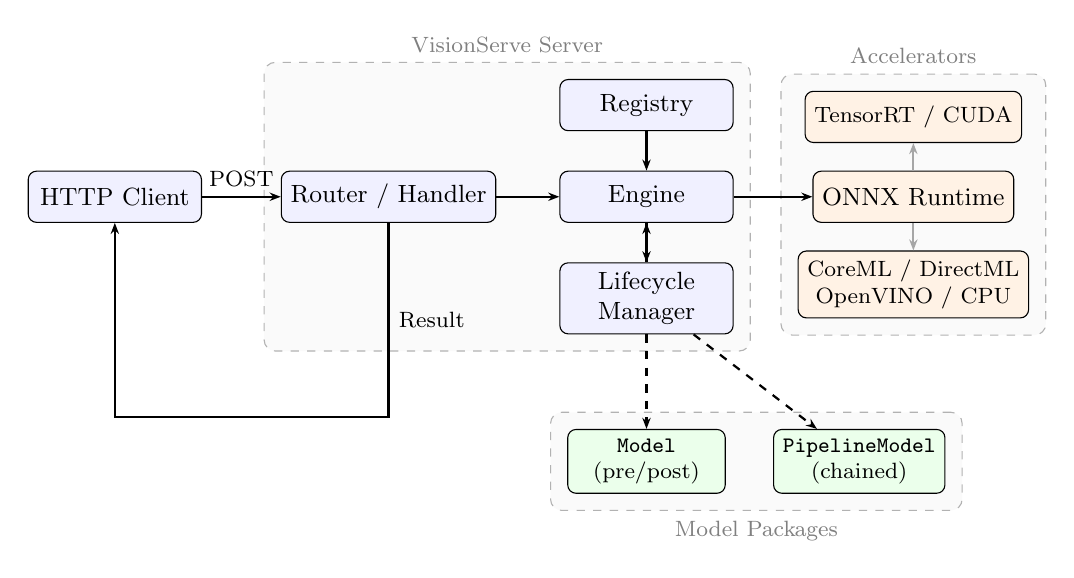
\begin{tikzpicture}[
      font=\small,
      node distance=0.55cm and 0.9cm,
      box/.style={draw, rounded corners=3pt, minimum width=2.2cm,
                  minimum height=0.65cm, align=center, fill=blue!6},
      ebox/.style={draw, rounded corners=3pt, minimum width=2.2cm,
                   minimum height=0.65cm, align=center, fill=orange!10},
      mbox/.style={draw, rounded corners=3pt, minimum width=2.0cm,
                   minimum height=0.58cm, align=center, fill=green!8,
                   font=\footnotesize},
      groupbox/.style={draw=gray!60, dashed, rounded corners=4pt,
                       inner sep=6pt, fill=gray!4},
      arr/.style={-{Stealth[length=4pt]}, thick},
  ]

  %% HTTP client
  \node[box] (client) {HTTP Client};

  %% Server internals group
  \node[box, right=1.0cm of client] (router)  {Router / Handler};
  \node[box, right=0.8cm of router] (engine)  {Engine};
  \node[box, above=0.5cm of engine] (registry){Registry};
  \node[box, below=0.5cm of engine] (lifecycle){Lifecycle\\Manager};

  \begin{scope}[on background layer]
    \node[groupbox, fit=(router)(registry)(lifecycle)(engine),
          label={[font=\footnotesize,gray]above:VisionServe Server}] (server) {};
  \end{scope}

  %% ORT group
  \node[ebox, right=1.0cm of engine] (ort) {ONNX Runtime};
  \node[ebox, above=0.35cm of ort,   font=\footnotesize] (ep1) {TensorRT / CUDA};
  \node[ebox, below=0.35cm of ort,   font=\footnotesize] (ep2) {CoreML / DirectML\\OpenVINO / CPU};

  \begin{scope}[on background layer]
    \node[groupbox, fit=(ort)(ep1)(ep2),
          label={[font=\footnotesize,gray]above:Accelerators}] (ortgroup) {};
  \end{scope}

  %% Model interface group (below Engine)
  \node[mbox, below=1.2cm of lifecycle] (mplain) {\texttt{Model}\\(pre/post)};
  \node[mbox, right=0.6cm of mplain]   (mpipe)  {\texttt{PipelineModel}\\(chained)};

  \begin{scope}[on background layer]
    \node[groupbox, fit=(mplain)(mpipe),
          label={[font=\footnotesize,gray]below:Model Packages}] (mgroup) {};
  \end{scope}

  %% Arrows
  \draw[arr] (client)   -- node[above,font=\footnotesize]{POST} (router);
  \draw[arr] (router)   -- (engine);
  \draw[arr] (registry) -- (engine);
  \draw[arr] (lifecycle)-- (engine);
  \draw[arr] (engine)   -- (ort);
  \draw[arr,gray!70] (ort) -- (ep1);
  \draw[arr,gray!70] (ort) -- (ep2);
  \draw[arr,dashed]  (engine)    -- (lifecycle);
  \draw[arr,dashed]  (lifecycle) -- (mplain);
  \draw[arr,dashed]  (lifecycle) -- (mpipe);
  \draw[arr] (router) -- node[right,font=\footnotesize]{Result} ++(0,-2.8) -| (client);

  \end{tikzpicture}
  \caption{High-level architecture of VisionServe.
           Solid arrows denote data flow; dashed arrows denote ownership or
           interface delegation.
           The Lifecycle Manager owns all ONNX sessions and is the sole
           gateway between model logic and the ONNX Runtime.}
  \label{fig:architecture}
\end{figure}

\subsection{Model Registry and Manifest}
\label{sec:design:registry}

Every model is described by a YAML manifest that declares all metadata
necessary for startup validation and session creation.
The mandatory fields are: \texttt{name} (unique identifier),
\texttt{task} (one of the six supported task types),
\texttt{license} (SPDX identifier),
\texttt{execution\_providers} (ordered list of preferred EPs),
preprocessing parameters (input resolution, normalisation statistics, and
letterbox strategy), and either a single \texttt{model\_file} path for
single-session models or a \texttt{files} map from role names to file paths
for multi-session models.
Roles are string keys agreed upon between the manifest and the model package:
for example, MobileSAM declares \texttt{encoder} and \texttt{decoder} roles;
Grounded-SAM declares \texttt{det}, \texttt{encoder}, and \texttt{decoder}.

At startup the registry parser reads every manifest in the model directory and
enforces the license allowlist: only \texttt{Apache-2.0}, \texttt{MIT}, and
BSD variants are accepted.
Any manifest bearing a non-allowlisted license --- including AGPL-3.0, as
carried by Ultralytics YOLO~\cite{ultralytics2023yolo,agpllicense} --- is
rejected with a descriptive error before any session is created.
This approach provides a strong audit boundary: downstream adopters can trust
that every model loaded by VisionServe carries a permissive license, regardless
of where the ONNX file was sourced.

\subsection{Lifecycle Management}
\label{sec:design:lifecycle}

ONNX Runtime sessions are expensive GPU resources: each session allocates
device memory proportional to model weight size and holds an execution context
that spans the full session lifetime.
Creating sessions on demand inside request handlers would cause repeated
allocation/deallocation cycles, unpredictable latency spikes, and potential
VRAM fragmentation.

\texttt{lifecycle.Manager} solves this by owning the full lifecycle of every
session.
At startup the manager creates one session per role per model, holds references
for the duration of the process, and releases them only on server shutdown.
Concurrent HTTP requests access sessions through a mutex-protected pool: a
request acquires a session handle, performs inference, and returns it to the
pool, ensuring that a session is never used by two goroutines simultaneously.
Neither model packages nor request handlers hold any reference to an ORT
session object; all access is mediated through the manager's typed API.
This single ownership invariant eliminates the most common class of
GPU resource leak in serving systems and is straightforward to audit.

\subsection{Model Interfaces}
\label{sec:design:interfaces}

VisionServe defines two Go interfaces that cover the full range of CV models.

\textbf{Model} is the interface for plain single-session models.
An implementation provides \texttt{Preprocess(img) (tensor, PreprocessMeta,
error)} and \texttt{Postprocess(output, meta) (Result, error)}.
The inference engine handles everything in between: it acquires a session
from the lifecycle manager, feeds the preprocessed tensor, collects the raw
output tensors, and calls \texttt{Postprocess}.
Model packages contain no inference code; they contain only numerical
transformations on image data and model output arrays.
This split keeps model packages testable in isolation --- unit tests exercise
pre/postprocess without an ONNX session --- and keeps the hot path in the
engine, where batching and concurrency controls can be applied uniformly.

\textbf{PipelineModel} is the interface for models that require a
\texttt{Prompt} (bounding box, point set, or text string) or that orchestrate
multiple ONNX sessions in sequence.
An implementation provides \texttt{Roles() []string}, which declares the role
keys the model expects in the session pool, and \texttt{Infer(img, prompt,
Runner) (Result, error)}, which drives the full pipeline.
The \texttt{Runner} gateway exposes a single method \texttt{Run(role, tensor)
([]Tensor, error)} that dispatches to the lifecycle manager by role name;
the pipeline model calls \texttt{Runner.Run} once per session in its chain and
assembles the final result.
Critically, the pipeline model never creates or frees sessions; it merely
names them.
This design supports arbitrarily deep chains --- GroundingDINO boxes flowing
into the MobileSAM encoder then decoder in Grounded-SAM --- without any
special-casing in the core engine.

\subsection{Unified Result Schema}
\label{sec:design:result}

All six task types return a single \texttt{Result} struct:
\begin{center}
\small
\texttt{Result\{task, model, Detections, Masks, Classifications,}\\
\texttt{DepthMap, Embeddings, DurationMs\}}
\end{center}
Fields irrelevant to a given task are null or empty.
\texttt{Detection} carries a \texttt{BBox} in the format \([x, y, w, h]\) in
\emph{original image coordinates}: the postprocess step uses the
\texttt{PreprocessMeta} produced during preprocessing --- which records the
original image dimensions and any letterbox padding offsets --- to map model-
space coordinates back to pixel-space before populating the result.
This mapping is done once, inside \texttt{Postprocess}, so no consumer of
\texttt{Result} ever needs to account for scaling or padding.

Masks are encoded as column-major (Fortran-order) run-length encoding (RLE) in
the COCO uncompressed style.
Column-major order matches the internal memory layout of SAM decoder outputs
and avoids a transpose when encoding, keeping the mask serialisation path
allocation-free.
A single schema simplifies client code: a generic display widget or
post-processing script works across all tasks without branching on task type.

\subsection{Execution Provider Fallback}
\label{sec:design:ep}

Hardware diversity is a defining constraint of edge CV deployment: the same
model may run on a Jetson module (TensorRT + CUDA), a developer laptop (CUDA
or CoreML), an Intel NUC (OpenVINO), or a Raspberry Pi (CPU only).
Rather than shipping separate binaries, VisionServe resolves this at session
creation time through a manifest-declared EP priority list such as
\texttt{[tensorrt, cuda, cpu]}.
The engine iterates the list in order; if ONNX Runtime reports that a given EP
is unavailable in the current ORT build, it is silently skipped and the next
is tried.
CPU is always appended as the final fallback regardless of what the manifest
declares, so inference always succeeds on any host.
The allowlisted EPs are: \texttt{tensorrt}, \texttt{cuda}, \texttt{coreml},
\texttt{directml}, \texttt{openvino}, and \texttt{cpu}; any EP name not in
this set is rejected at manifest parse time to prevent misconfiguration.
The fallback chain is fully transparent: the \texttt{Result} struct records
which EP was ultimately selected, so operators can verify hardware utilisation
without inspecting logs.


% -----------------------------------------------------------------------
\section{Model Catalog}
\label{sec:catalog}
% catalog.tex — Section 4: Model Catalog
% Included by main.tex as % catalog.tex — Section 4: Model Catalog
% Included by main.tex as % catalog.tex — Section 4: Model Catalog
% Included by main.tex as \input{sections/catalog}
% No \begin{document} / \end{document}

\subsection{Task Types}
\label{sec:catalog:tasks}

VisionServe organises its model portfolio around seven computer-vision task types.
Table~\ref{tab:task-types} defines each type, states the expected input and output
contract, and names representative models currently registered in the system.

\begin{table*}[t]
  \centering
  \small
  \caption{Task types supported by VisionServe.}
  \label{tab:task-types}
  \begin{tabular}{llp{6.2cm}l}
    \toprule
    \textbf{Task} & \textbf{I/O Contract} & \textbf{Description} & \textbf{Example Models} \\
    \midrule
    \texttt{detection}     & image $\to$ boxes     &
      Localise and classify objects in an image.
      Returns axis-aligned bounding boxes in original-image coordinates
      together with class labels and confidence scores.
      &
      RF-DETR, SCRFD, PaddleOCR \\[4pt]

    \texttt{segmentation}  & image + prompt $\to$ masks &
      Produce per-pixel binary masks, optionally conditioned on a box or
      point prompt.  Masks are encoded as column-major run-length encoding
      (RLE) in the unified \texttt{Result} schema.
      &
      MobileSAM, EfficientSAM, SAM2 \\[4pt]

    \texttt{open\_vocab}   & image + text $\to$ boxes &
      Detect objects whose categories are specified as free-form natural-language
      queries at request time, without any fixed class vocabulary.
      &
      GroundingDINO \\[4pt]

    \texttt{classification}& image $\to$ label + score &
      Assign a single top-\(k\) label from a closed-set vocabulary
      (e.g.\ ImageNet-1k) to the entire image.
      &
      EfficientNet-B0, MobileNetV3 \\[4pt]

    \texttt{depth}         & image $\to$ depth map &
      Estimate a per-pixel relative or metric depth map.  Output is a
      single-channel float32 tensor aligned to the input resolution.
      &
      MiDaS, Depth Anything V2 \\[4pt]

    \texttt{embed}         & image $\to$ vector &
      Extract a compact, semantically rich embedding vector suitable for
      retrieval, zero-shot classification, or downstream ML pipelines.
      &
      CLIP ViT-B/32 \\[4pt]

    \texttt{grasp}         & image $\to$ grasps &
      Synthesise planar parallel-jaw grasps ($(x,y,\theta,\text{width},\text{quality})$ in
      original-image coordinates) from a segmentation mask via a pure-Go analytic
      antipodal force-closure search (no extra ONNX weights).  Class-agnostic
      (whole-image automask) or class-aware (detector $\to$ mask $\to$ grasp).
      &
      grasp, grasp-rfdetr, grasp-gd \\
    \bottomrule
  \end{tabular}
\end{table*}

\subsection{Model Inventory}
\label{sec:catalog:inventory}

Table~\ref{tab:model-inventory} enumerates all 19 models in the current VisionServe
registry.  Each model is distributed as one or more ONNX files; multi-session models
(MobileSAM, EfficientSAM, SAM2, Grounded-SAM, and the grasp pipelines) use the
\texttt{PipelineModel} interface and declare a \texttt{files:} role map in their manifest.
The three grasp pipelines reuse the segmentation/detection weights of sibling models and add
no new ONNX file: the grasp synthesis itself is a pure-Go analytic stage.

\begin{table*}[t]
  \centering
  \small
  \caption{%
    VisionServe model inventory.
    Architecture notes describe the primary network family.
    Models marked $\dagger$ are pending benchmark runs (see text).%
  }
  \label{tab:model-inventory}
  \begin{tabular}{llll}
    \toprule
    \textbf{Model} & \textbf{Task} & \textbf{License} & \textbf{Architecture} \\
    \midrule
    \texttt{rf-detr}          & detection     & Apache-2.0 & ResNet-50 backbone + DETR head (NMS-free) \\
    \texttt{rf-detr-nano}     & detection     & Apache-2.0 & Lightweight DETR variant \\
    \texttt{rt-detr}$^\dagger$& detection     & Apache-2.0 & Hybrid CNN/Transformer real-time DETR \\
    \texttt{scrfd}            & detection     & MIT        & Sample- \& computation-redistributed face detector \\
    \texttt{paddle-ocr}       & detection     & Apache-2.0 & PP-OCRv4 text detection backbone \\
    \texttt{grounding-dino}   & open\_vocab   & Apache-2.0 & Swin-T image encoder + BERT text encoder \\
    \texttt{mobile-sam}       & segmentation  & Apache-2.0 & Tiny ViT encoder + SAM decoder \\
    \texttt{efficient-sam}    & segmentation  & Apache-2.0 & ViT-S/16 encoder with masked-image pretraining \\
    \texttt{sam2}             & segmentation  & Apache-2.0 & Hiera-Tiny image/video encoder + SAM2 decoder \\
    \texttt{nano-sam}$^\dagger$& segmentation & Apache-2.0 & ResNet-18 distilled SAM encoder \\
    \texttt{grounded-sam}    & open\_vocab    & Apache-2.0 & GroundingDINO boxes $\to$ MobileSAM masks (composite) \\
    \texttt{midas}            & depth         & MIT        & DPT-Hybrid (ViT-H + dense prediction transformer) \\
    \texttt{depth-anything-v2}$^\dagger$ & depth & Apache-2.0 & ViT-S teacher-student depth foundation model \\
    \texttt{efficientnet-b0}  & classification& Apache-2.0 & EfficientNet-B0 compound-scaled CNN \\
    \texttt{mobilenet-v3}     & classification& Apache-2.0 & MobileNetV3-Large depthwise-separable CNN \\
    \texttt{clip}             & embed         & MIT        & CLIP ViT-B/32 vision encoder (image side only) \\
    \texttt{grasp}            & grasp         & Apache-2.0 & MobileSAM automask $\to$ pure-Go analytic grasps (class-agnostic) \\
    \texttt{grasp-rfdetr}     & grasp         & Apache-2.0 & RF-DETR boxes $\to$ MobileSAM $\to$ analytic grasps (class-aware) \\
    \texttt{grasp-gd}         & grasp         & Apache-2.0 & GroundingDINO boxes $\to$ MobileSAM $\to$ analytic grasps (text-prompted) \\
    \bottomrule
  \end{tabular}
\end{table*}

\noindent
Three models marked $\dagger$ remain pending: \texttt{rt-detr} and
\texttt{depth-anything-v2} require authenticated HuggingFace downloads, and
\texttt{nano-sam} requires a manual ONNX export.  All four grasp/composite pipelines
(\texttt{grasp}, \texttt{grasp-rfdetr}, \texttt{grounded-sam}, \texttt{grasp-gd}) are now
benchmarked (Section~\ref{sec:eval:latency}); the two GroundingDINO-based pipelines are
serialized for concurrency-safety (a fixed \texttt{SA\_ONSTACK} crash, Section~\ref{sec:limitations})
and are reported single-stream.

\paragraph{Grasp and license discipline.}
The grasp capability also illustrates why the license gate (C1) is load-bearing rather than
decorative.  In selecting a grasp method we rejected the most accurate learned grasp
models, GQ-CNN / FC-GQ-CNN (Dex-Net), under a UC~Berkeley ``educational, research, and
not-for-profit'' license, because that non-commercial bar is incompatible with
VisionServe's permissive, commercial-friendly stance, as AGPL is.  The shipped path
instead pairs a permissive MobileSAM mask with a clean-room pure-Go analytic synthesizer (no
weights, no license at all), so the seventh task adds capability without adding license risk.

\subsection{License Safety}
\label{sec:catalog:license}

Open-source computer-vision models carry heterogeneous licenses, and the distinction
between permissive and copyleft licenses has material consequences for downstream
deployments.  The most prominent example is the Ultralytics YOLO family
\cite{ultralytics2023yolo}, which is released under the GNU Affero General
Public License v3.0 (AGPL-3.0) \cite{agpllicense}.  AGPL-3.0 extends the GPL copyleft
to networked services: any software that uses AGPL code and provides access to
users over a network must release its entire source under AGPL-3.0.  As a result,
integrating a single AGPL model into an inference server would virally relicense the
server (and every product built on it) under AGPL-3.0.  This is incompatible with
closed-source, proprietary, or commercial deployments; the only escape is a separate
commercial license negotiated with the copyright holder.

VisionServe enforces an allowlist of permissive licenses
(\texttt{Apache-2.0}, \texttt{MIT}, \texttt{BSD-2-Clause}, \texttt{BSD-3-Clause})
in the registry parser at process startup \cite{apachelicense}.  Any model manifest
that declares a \texttt{license} field outside this allowlist causes the server to
abort with a clear error message, preventing accidental integration of copyleft models.
This check is implemented in code, not merely documented: the manifest
\texttt{license} field is a required string, and the parser rejects absent or
non-allowlisted values before any ONNX session is initialised.  This design choice is
deliberate: because VisionServe is itself Apache-2.0 and targets edge deployments in
commercial and closed-source products, its permissive character must be preserved by
every model it ships.

\paragraph{Threat model.}
We scope the license gate (contribution~C1), since its value depends on
stating both what it defends against and what it cannot.
\emph{In scope.}  The gate is designed to prevent four failure modes at the moment the
runtime loads model weights:
(i)~accidentally loading a copyleft (AGPL) model that would virally relicense an otherwise
permissive deployment;
(ii)~``permissive-washing'' or license drift, where a model's restrictive license is
silently dropped or relabelled as permissive on the way into the deployment;
(iii)~tampered or swapped weight bytes that no longer correspond to the audited model
(a content mismatch);
(iv)~weights pulled from an unvetted origin; and
(v)~a manifest relabelled by its author with a permissive-but-wrong license that diverges from
the maintainer-audited upstream (caught by the provenance ledger, which the allowlist alone
cannot detect because the wrong label is itself permissive).
\emph{Mechanism.}  Enforcement is entirely offline, in a single binary, and consists of
four bound checks applied at load time.
First, the declared \texttt{license} field must be in the permissive allowlist
(\texttt{Apache-2.0}/\texttt{MIT}/\texttt{BSD}); the registry parser
(\texttt{Manifest.validate()}) refuses any other value before a session is created.
Second, the SHA-256 digest of the weight bytes must equal the digest declared in the
manifest (\texttt{Manifest.VerifyWeights()}); a mismatch refuses the load.
Third, when a verified-source allowlist is supplied, the manifest's \texttt{source\_url}
must fall under an audited prefix.
Fourth, the check that closes the upstream-relabelling hole for the curated
catalog: in the opt-in verified mode the contributor-declared license must equal the
license recorded for that \texttt{source\_url} prefix in a \emph{maintainer-audited
license-provenance ledger} (\texttt{Manifest.VerifyLicenseProvenance()}).  The ledger is a
separate in-binary table in which a maintainer records, per audited upstream, the SPDX license
they verified by reading the upstream's actual LICENSE file, the URL of that file, and its
SHA-256 as evidence.  Because contributors edit manifests and maintainers edit the ledger, the
two authorities are separated: a pull request that flips a manifest's \texttt{license} to
sneak in a copyleft model is refused by a record the PR author does not control.  Together these
checks bind a declared-permissive license to specific audited bytes, an audited origin,
and an independent audited record of the upstream's true license, without any network call.
\emph{Out of scope.}  The allowlist and SHA-256/source pins alone still trust the declared
license string and mitigate only substitution (swapped bytes, wrong mirror), not
upstream mislabelling; the ledger removes that residue for the shipped catalog by
cross-checking against an independent human audit.  What remains out of scope is genuine: the
ledger's ground truth is a one-time human audit of the upstream LICENSE file (a re-audit detects
later divergence via the pinned LICENSE-file hash, but an upstream mislabelled at audit
time is not caught), and it covers only audited upstreams, not arbitrary un-audited uploads, for
which a universal license oracle is impossible.  We therefore frame~C1 as load-time
license-policy enforcement, hardened by content-hashing, a verified-source pin, and an
audited provenance ledger: strong for the curated catalog, and not a
machine-checkable license guarantee for arbitrary models.
\emph{Why existing layers do not cover it.}  As discussed in
Section~\ref{sec:related}, build-time software-composition-analysis scanners
(ScanCode, FOSSology, Snyk) operate on source dependency trees and emit reports, not a
load-time decision over weights; deploy-time admission controllers (Kyverno, OPA
Gatekeeper, Sigstore policy-controller) verify container-image signatures at pod
admission, i.e.\ container integrity, not a license policy over model weights; and model
signing (OpenSSF/Sigstore) proves signer identity and byte integrity, not license policy.
None of these enforces a license policy at the moment the runtime loads model weights,
offline, which is the gap~C1 fills.

\paragraph{Adversarial demonstration.}
To show that the gate refuses bad models rather than merely documenting an
intent to, Table~\ref{tab:gate} reports a reproducible adversarial demonstration.
Starting from a baseline manifest (permissive license, correct SHA-256, audited source)
that is admitted, we apply one adversarial mutation at a time and record the gate's
verdict.  Each mutation maps to one of the four bound checks above, and each is refused
with the runtime's own diagnostic message.  The six cases are exercised by the test
\texttt{TestGate\_AdversarialDemo}; the transcript is reproducible via
\texttt{go test ./internal/registry -run TestGate\_AdversarialDemo -v}.

\begin{table}[t]
  \centering
  \footnotesize
  \setlength{\tabcolsep}{3pt}
  \caption{%
    Reproducible adversarial demonstration of the load-time license gate (C1).
    Starting from an admitted baseline, each row applies one manifest mutation and
    records the runtime's verdict and (abbreviated) diagnostic.  Reproducible via
    \texttt{go test ./internal/registry -run TestGate\_AdversarialDemo -v}
    (\texttt{internal/registry/gate\_demo\_test.go}); the long digest is abbreviated
    with \(\dots\) and the temporary weight path is shown as \texttt{<model.onnx>}.%
  }
  \label{tab:gate}
  \begin{tabular}{p{1.2cm}p{1.5cm}p{5.4cm}}
    \toprule
    \textbf{Condition} & \textbf{Manifest change} & \textbf{Gate outcome} \\
    \midrule
    Baseline &
      permissive license \mbox{+} correct SHA-256 \mbox{+} audited source &
      \textbf{ADMITTED}: \texttt{license=Apache-2.0}, sha256 bound to bytes, source under
      audited prefix \\[4pt]

    Relabel license &
      \texttt{license = AGPL-3.0} &
      \textbf{REFUSED (license)}: \texttt{license "AGPL-3.0" is not allowed --- only
      permissive licenses accepted (Apache-2.0/MIT/BSD); AGPL is strictly forbidden} \\[4pt]

    Byte-swap weights &
      weights \(\neq\) declared SHA-256 &
      \textbf{REFUSED (hash)}: \texttt{sha256 mismatch for <model.onnx>: manifest declares
      aaaa\(\dots\)aaaa but file is 0b4895d0\(\dots\)29bb57 --- refusing to load (the
      declared license is bound to the audited bytes)} \\[4pt]

    Wrong origin &
      \texttt{source\_url} outside allowlist &
      \textbf{REFUSED (source)}: \texttt{source\_url
      "https://random-mirror.\allowbreak example.com/x.onnx" is not under any audited prefix in the
      verified-source allowlist} \\[4pt]

    Relabel vs.\ ledger &
      permissive but \texttt{license=MIT} where ledger says \texttt{Apache-2.0} &
      \textbf{REFUSED (ledger)}: \texttt{declared license "MIT" does not match the
      maintainer-audited upstream license "Apache-2.0" \dots\ (manifest may be mislabeled or
      relicensed)}; the allowlist cannot catch this (MIT is permissive), only the ledger does \\[4pt]

    Un-audited upstream &
      \texttt{source\_url} with no ledger entry &
      \textbf{REFUSED (ledger)}: \texttt{\dots\ has no maintainer-audited license-ledger entry
      (verified mode requires an audited upstream)} \\
    \bottomrule
  \end{tabular}
\end{table}

\subsection{Manifest Specification}
\label{sec:catalog:manifest}

Each model is described by a YAML \emph{manifest} file that the registry loads at
startup.  The manifest declares all information needed to validate the license,
locate ONNX artefacts, configure the execution-provider fallback chain, and pass
preprocessing parameters to the model's Go package without hard-coding them.

For plain (single-session) models, the manifest provides a single \texttt{model\_file}
path.  For \texttt{PipelineModel} instances that require multiple ONNX sessions
(e.g.\ MobileSAM encoder/decoder, Grounded-SAM), the manifest uses a \texttt{files:}
role map instead; each key is a logical role name that the model package uses to
request the correct session from \texttt{lifecycle.Manager}.

The following listing shows a representative manifest for \texttt{rf-detr-nano}:

\begin{lstlisting}[language=yaml, float=tbp, caption={Sample manifest: \texttt{rf-detr-nano}.},
                   label={lst:manifest}]
name: rf-detr-nano
task: detection
license: Apache-2.0
source_url: https://huggingface.co/PierreMarieCurie/.../rf-detr-nano.onnx
sha256: 3fcbba0f...be67abb2   # binds license to these exact bytes (verified mode)

execution_providers:
  - tensorrt
  - cuda
  - cpu

model_file: models/rf_detr_nano.onnx

preprocessing:
  resize: [560, 560]
  mean:   [0.485, 0.456, 0.406]
  std:    [0.229, 0.224, 0.225]
  input_format: NCHW
\end{lstlisting}

\noindent
The \texttt{execution\_providers} list is tried in order; if the ORT build on the host
does not include a listed provider, it is skipped silently and the next entry is
attempted.  \texttt{cpu} is always appended last to guarantee a functional fallback on
any hardware.  The \texttt{preprocessing} block is parsed into a \texttt{PreprocessMeta}
struct and passed to the model's \texttt{Preprocess} method, ensuring that bounding-box
coordinates are mapped back to original-image space before the result is serialised.

% No \begin{document} / \end{document}

\subsection{Task Types}
\label{sec:catalog:tasks}

VisionServe organises its model portfolio around seven computer-vision task types.
Table~\ref{tab:task-types} defines each type, states the expected input and output
contract, and names representative models currently registered in the system.

\begin{table*}[t]
  \centering
  \small
  \caption{Task types supported by VisionServe.}
  \label{tab:task-types}
  \begin{tabular}{llp{6.2cm}l}
    \toprule
    \textbf{Task} & \textbf{I/O Contract} & \textbf{Description} & \textbf{Example Models} \\
    \midrule
    \texttt{detection}     & image $\to$ boxes     &
      Localise and classify objects in an image.
      Returns axis-aligned bounding boxes in original-image coordinates
      together with class labels and confidence scores.
      &
      RF-DETR, SCRFD, PaddleOCR \\[4pt]

    \texttt{segmentation}  & image + prompt $\to$ masks &
      Produce per-pixel binary masks, optionally conditioned on a box or
      point prompt.  Masks are encoded as column-major run-length encoding
      (RLE) in the unified \texttt{Result} schema.
      &
      MobileSAM, EfficientSAM, SAM2 \\[4pt]

    \texttt{open\_vocab}   & image + text $\to$ boxes &
      Detect objects whose categories are specified as free-form natural-language
      queries at request time, without any fixed class vocabulary.
      &
      GroundingDINO \\[4pt]

    \texttt{classification}& image $\to$ label + score &
      Assign a single top-\(k\) label from a closed-set vocabulary
      (e.g.\ ImageNet-1k) to the entire image.
      &
      EfficientNet-B0, MobileNetV3 \\[4pt]

    \texttt{depth}         & image $\to$ depth map &
      Estimate a per-pixel relative or metric depth map.  Output is a
      single-channel float32 tensor aligned to the input resolution.
      &
      MiDaS, Depth Anything V2 \\[4pt]

    \texttt{embed}         & image $\to$ vector &
      Extract a compact, semantically rich embedding vector suitable for
      retrieval, zero-shot classification, or downstream ML pipelines.
      &
      CLIP ViT-B/32 \\[4pt]

    \texttt{grasp}         & image $\to$ grasps &
      Synthesise planar parallel-jaw grasps ($(x,y,\theta,\text{width},\text{quality})$ in
      original-image coordinates) from a segmentation mask via a pure-Go analytic
      antipodal force-closure search (no extra ONNX weights).  Class-agnostic
      (whole-image automask) or class-aware (detector $\to$ mask $\to$ grasp).
      &
      grasp, grasp-rfdetr, grasp-gd \\
    \bottomrule
  \end{tabular}
\end{table*}

\subsection{Model Inventory}
\label{sec:catalog:inventory}

Table~\ref{tab:model-inventory} enumerates all 19 models in the current VisionServe
registry.  Each model is distributed as one or more ONNX files; multi-session models
(MobileSAM, EfficientSAM, SAM2, Grounded-SAM, and the grasp pipelines) use the
\texttt{PipelineModel} interface and declare a \texttt{files:} role map in their manifest.
The three grasp pipelines reuse the segmentation/detection weights of sibling models and add
no new ONNX file: the grasp synthesis itself is a pure-Go analytic stage.

\begin{table*}[t]
  \centering
  \small
  \caption{%
    VisionServe model inventory.
    Architecture notes describe the primary network family.
    Models marked $\dagger$ are pending benchmark runs (see text).%
  }
  \label{tab:model-inventory}
  \begin{tabular}{llll}
    \toprule
    \textbf{Model} & \textbf{Task} & \textbf{License} & \textbf{Architecture} \\
    \midrule
    \texttt{rf-detr}          & detection     & Apache-2.0 & ResNet-50 backbone + DETR head (NMS-free) \\
    \texttt{rf-detr-nano}     & detection     & Apache-2.0 & Lightweight DETR variant \\
    \texttt{rt-detr}$^\dagger$& detection     & Apache-2.0 & Hybrid CNN/Transformer real-time DETR \\
    \texttt{scrfd}            & detection     & MIT        & Sample- \& computation-redistributed face detector \\
    \texttt{paddle-ocr}       & detection     & Apache-2.0 & PP-OCRv4 text detection backbone \\
    \texttt{grounding-dino}   & open\_vocab   & Apache-2.0 & Swin-T image encoder + BERT text encoder \\
    \texttt{mobile-sam}       & segmentation  & Apache-2.0 & Tiny ViT encoder + SAM decoder \\
    \texttt{efficient-sam}    & segmentation  & Apache-2.0 & ViT-S/16 encoder with masked-image pretraining \\
    \texttt{sam2}             & segmentation  & Apache-2.0 & Hiera-Tiny image/video encoder + SAM2 decoder \\
    \texttt{nano-sam}$^\dagger$& segmentation & Apache-2.0 & ResNet-18 distilled SAM encoder \\
    \texttt{grounded-sam}    & open\_vocab    & Apache-2.0 & GroundingDINO boxes $\to$ MobileSAM masks (composite) \\
    \texttt{midas}            & depth         & MIT        & DPT-Hybrid (ViT-H + dense prediction transformer) \\
    \texttt{depth-anything-v2}$^\dagger$ & depth & Apache-2.0 & ViT-S teacher-student depth foundation model \\
    \texttt{efficientnet-b0}  & classification& Apache-2.0 & EfficientNet-B0 compound-scaled CNN \\
    \texttt{mobilenet-v3}     & classification& Apache-2.0 & MobileNetV3-Large depthwise-separable CNN \\
    \texttt{clip}             & embed         & MIT        & CLIP ViT-B/32 vision encoder (image side only) \\
    \texttt{grasp}            & grasp         & Apache-2.0 & MobileSAM automask $\to$ pure-Go analytic grasps (class-agnostic) \\
    \texttt{grasp-rfdetr}     & grasp         & Apache-2.0 & RF-DETR boxes $\to$ MobileSAM $\to$ analytic grasps (class-aware) \\
    \texttt{grasp-gd}         & grasp         & Apache-2.0 & GroundingDINO boxes $\to$ MobileSAM $\to$ analytic grasps (text-prompted) \\
    \bottomrule
  \end{tabular}
\end{table*}

\noindent
Three models marked $\dagger$ remain pending: \texttt{rt-detr} and
\texttt{depth-anything-v2} require authenticated HuggingFace downloads, and
\texttt{nano-sam} requires a manual ONNX export.  All four grasp/composite pipelines
(\texttt{grasp}, \texttt{grasp-rfdetr}, \texttt{grounded-sam}, \texttt{grasp-gd}) are now
benchmarked (Section~\ref{sec:eval:latency}); the two GroundingDINO-based pipelines are
serialized for concurrency-safety (a fixed \texttt{SA\_ONSTACK} crash, Section~\ref{sec:limitations})
and are reported single-stream.

\paragraph{Grasp and license discipline.}
The grasp capability also illustrates why the license gate (C1) is load-bearing rather than
decorative.  In selecting a grasp method we rejected the most accurate learned grasp
models, GQ-CNN / FC-GQ-CNN (Dex-Net), under a UC~Berkeley ``educational, research, and
not-for-profit'' license, because that non-commercial bar is incompatible with
VisionServe's permissive, commercial-friendly stance, as AGPL is.  The shipped path
instead pairs a permissive MobileSAM mask with a clean-room pure-Go analytic synthesizer (no
weights, no license at all), so the seventh task adds capability without adding license risk.

\subsection{License Safety}
\label{sec:catalog:license}

Open-source computer-vision models carry heterogeneous licenses, and the distinction
between permissive and copyleft licenses has material consequences for downstream
deployments.  The most prominent example is the Ultralytics YOLO family
\cite{ultralytics2023yolo}, which is released under the GNU Affero General
Public License v3.0 (AGPL-3.0) \cite{agpllicense}.  AGPL-3.0 extends the GPL copyleft
to networked services: any software that uses AGPL code and provides access to
users over a network must release its entire source under AGPL-3.0.  As a result,
integrating a single AGPL model into an inference server would virally relicense the
server (and every product built on it) under AGPL-3.0.  This is incompatible with
closed-source, proprietary, or commercial deployments; the only escape is a separate
commercial license negotiated with the copyright holder.

VisionServe enforces an allowlist of permissive licenses
(\texttt{Apache-2.0}, \texttt{MIT}, \texttt{BSD-2-Clause}, \texttt{BSD-3-Clause})
in the registry parser at process startup \cite{apachelicense}.  Any model manifest
that declares a \texttt{license} field outside this allowlist causes the server to
abort with a clear error message, preventing accidental integration of copyleft models.
This check is implemented in code, not merely documented: the manifest
\texttt{license} field is a required string, and the parser rejects absent or
non-allowlisted values before any ONNX session is initialised.  This design choice is
deliberate: because VisionServe is itself Apache-2.0 and targets edge deployments in
commercial and closed-source products, its permissive character must be preserved by
every model it ships.

\paragraph{Threat model.}
We scope the license gate (contribution~C1), since its value depends on
stating both what it defends against and what it cannot.
\emph{In scope.}  The gate is designed to prevent four failure modes at the moment the
runtime loads model weights:
(i)~accidentally loading a copyleft (AGPL) model that would virally relicense an otherwise
permissive deployment;
(ii)~``permissive-washing'' or license drift, where a model's restrictive license is
silently dropped or relabelled as permissive on the way into the deployment;
(iii)~tampered or swapped weight bytes that no longer correspond to the audited model
(a content mismatch);
(iv)~weights pulled from an unvetted origin; and
(v)~a manifest relabelled by its author with a permissive-but-wrong license that diverges from
the maintainer-audited upstream (caught by the provenance ledger, which the allowlist alone
cannot detect because the wrong label is itself permissive).
\emph{Mechanism.}  Enforcement is entirely offline, in a single binary, and consists of
four bound checks applied at load time.
First, the declared \texttt{license} field must be in the permissive allowlist
(\texttt{Apache-2.0}/\texttt{MIT}/\texttt{BSD}); the registry parser
(\texttt{Manifest.validate()}) refuses any other value before a session is created.
Second, the SHA-256 digest of the weight bytes must equal the digest declared in the
manifest (\texttt{Manifest.VerifyWeights()}); a mismatch refuses the load.
Third, when a verified-source allowlist is supplied, the manifest's \texttt{source\_url}
must fall under an audited prefix.
Fourth, the check that closes the upstream-relabelling hole for the curated
catalog: in the opt-in verified mode the contributor-declared license must equal the
license recorded for that \texttt{source\_url} prefix in a \emph{maintainer-audited
license-provenance ledger} (\texttt{Manifest.VerifyLicenseProvenance()}).  The ledger is a
separate in-binary table in which a maintainer records, per audited upstream, the SPDX license
they verified by reading the upstream's actual LICENSE file, the URL of that file, and its
SHA-256 as evidence.  Because contributors edit manifests and maintainers edit the ledger, the
two authorities are separated: a pull request that flips a manifest's \texttt{license} to
sneak in a copyleft model is refused by a record the PR author does not control.  Together these
checks bind a declared-permissive license to specific audited bytes, an audited origin,
and an independent audited record of the upstream's true license, without any network call.
\emph{Out of scope.}  The allowlist and SHA-256/source pins alone still trust the declared
license string and mitigate only substitution (swapped bytes, wrong mirror), not
upstream mislabelling; the ledger removes that residue for the shipped catalog by
cross-checking against an independent human audit.  What remains out of scope is genuine: the
ledger's ground truth is a one-time human audit of the upstream LICENSE file (a re-audit detects
later divergence via the pinned LICENSE-file hash, but an upstream mislabelled at audit
time is not caught), and it covers only audited upstreams, not arbitrary un-audited uploads, for
which a universal license oracle is impossible.  We therefore frame~C1 as load-time
license-policy enforcement, hardened by content-hashing, a verified-source pin, and an
audited provenance ledger: strong for the curated catalog, and not a
machine-checkable license guarantee for arbitrary models.
\emph{Why existing layers do not cover it.}  As discussed in
Section~\ref{sec:related}, build-time software-composition-analysis scanners
(ScanCode, FOSSology, Snyk) operate on source dependency trees and emit reports, not a
load-time decision over weights; deploy-time admission controllers (Kyverno, OPA
Gatekeeper, Sigstore policy-controller) verify container-image signatures at pod
admission, i.e.\ container integrity, not a license policy over model weights; and model
signing (OpenSSF/Sigstore) proves signer identity and byte integrity, not license policy.
None of these enforces a license policy at the moment the runtime loads model weights,
offline, which is the gap~C1 fills.

\paragraph{Adversarial demonstration.}
To show that the gate refuses bad models rather than merely documenting an
intent to, Table~\ref{tab:gate} reports a reproducible adversarial demonstration.
Starting from a baseline manifest (permissive license, correct SHA-256, audited source)
that is admitted, we apply one adversarial mutation at a time and record the gate's
verdict.  Each mutation maps to one of the four bound checks above, and each is refused
with the runtime's own diagnostic message.  The six cases are exercised by the test
\texttt{TestGate\_AdversarialDemo}; the transcript is reproducible via
\texttt{go test ./internal/registry -run TestGate\_AdversarialDemo -v}.

\begin{table}[t]
  \centering
  \footnotesize
  \setlength{\tabcolsep}{3pt}
  \caption{%
    Reproducible adversarial demonstration of the load-time license gate (C1).
    Starting from an admitted baseline, each row applies one manifest mutation and
    records the runtime's verdict and (abbreviated) diagnostic.  Reproducible via
    \texttt{go test ./internal/registry -run TestGate\_AdversarialDemo -v}
    (\texttt{internal/registry/gate\_demo\_test.go}); the long digest is abbreviated
    with \(\dots\) and the temporary weight path is shown as \texttt{<model.onnx>}.%
  }
  \label{tab:gate}
  \begin{tabular}{p{1.2cm}p{1.5cm}p{5.4cm}}
    \toprule
    \textbf{Condition} & \textbf{Manifest change} & \textbf{Gate outcome} \\
    \midrule
    Baseline &
      permissive license \mbox{+} correct SHA-256 \mbox{+} audited source &
      \textbf{ADMITTED}: \texttt{license=Apache-2.0}, sha256 bound to bytes, source under
      audited prefix \\[4pt]

    Relabel license &
      \texttt{license = AGPL-3.0} &
      \textbf{REFUSED (license)}: \texttt{license "AGPL-3.0" is not allowed --- only
      permissive licenses accepted (Apache-2.0/MIT/BSD); AGPL is strictly forbidden} \\[4pt]

    Byte-swap weights &
      weights \(\neq\) declared SHA-256 &
      \textbf{REFUSED (hash)}: \texttt{sha256 mismatch for <model.onnx>: manifest declares
      aaaa\(\dots\)aaaa but file is 0b4895d0\(\dots\)29bb57 --- refusing to load (the
      declared license is bound to the audited bytes)} \\[4pt]

    Wrong origin &
      \texttt{source\_url} outside allowlist &
      \textbf{REFUSED (source)}: \texttt{source\_url
      "https://random-mirror.\allowbreak example.com/x.onnx" is not under any audited prefix in the
      verified-source allowlist} \\[4pt]

    Relabel vs.\ ledger &
      permissive but \texttt{license=MIT} where ledger says \texttt{Apache-2.0} &
      \textbf{REFUSED (ledger)}: \texttt{declared license "MIT" does not match the
      maintainer-audited upstream license "Apache-2.0" \dots\ (manifest may be mislabeled or
      relicensed)}; the allowlist cannot catch this (MIT is permissive), only the ledger does \\[4pt]

    Un-audited upstream &
      \texttt{source\_url} with no ledger entry &
      \textbf{REFUSED (ledger)}: \texttt{\dots\ has no maintainer-audited license-ledger entry
      (verified mode requires an audited upstream)} \\
    \bottomrule
  \end{tabular}
\end{table}

\subsection{Manifest Specification}
\label{sec:catalog:manifest}

Each model is described by a YAML \emph{manifest} file that the registry loads at
startup.  The manifest declares all information needed to validate the license,
locate ONNX artefacts, configure the execution-provider fallback chain, and pass
preprocessing parameters to the model's Go package without hard-coding them.

For plain (single-session) models, the manifest provides a single \texttt{model\_file}
path.  For \texttt{PipelineModel} instances that require multiple ONNX sessions
(e.g.\ MobileSAM encoder/decoder, Grounded-SAM), the manifest uses a \texttt{files:}
role map instead; each key is a logical role name that the model package uses to
request the correct session from \texttt{lifecycle.Manager}.

The following listing shows a representative manifest for \texttt{rf-detr-nano}:

\begin{lstlisting}[language=yaml, float=tbp, caption={Sample manifest: \texttt{rf-detr-nano}.},
                   label={lst:manifest}]
name: rf-detr-nano
task: detection
license: Apache-2.0
source_url: https://huggingface.co/PierreMarieCurie/.../rf-detr-nano.onnx
sha256: 3fcbba0f...be67abb2   # binds license to these exact bytes (verified mode)

execution_providers:
  - tensorrt
  - cuda
  - cpu

model_file: models/rf_detr_nano.onnx

preprocessing:
  resize: [560, 560]
  mean:   [0.485, 0.456, 0.406]
  std:    [0.229, 0.224, 0.225]
  input_format: NCHW
\end{lstlisting}

\noindent
The \texttt{execution\_providers} list is tried in order; if the ORT build on the host
does not include a listed provider, it is skipped silently and the next entry is
attempted.  \texttt{cpu} is always appended last to guarantee a functional fallback on
any hardware.  The \texttt{preprocessing} block is parsed into a \texttt{PreprocessMeta}
struct and passed to the model's \texttt{Preprocess} method, ensuring that bounding-box
coordinates are mapped back to original-image space before the result is serialised.

% No \begin{document} / \end{document}

\subsection{Task Types}
\label{sec:catalog:tasks}

VisionServe organises its model portfolio around seven computer-vision task types.
Table~\ref{tab:task-types} defines each type, states the expected input and output
contract, and names representative models currently registered in the system.

\begin{table*}[t]
  \centering
  \small
  \caption{Task types supported by VisionServe.}
  \label{tab:task-types}
  \begin{tabular}{llp{6.2cm}l}
    \toprule
    \textbf{Task} & \textbf{I/O Contract} & \textbf{Description} & \textbf{Example Models} \\
    \midrule
    \texttt{detection}     & image $\to$ boxes     &
      Localise and classify objects in an image.
      Returns axis-aligned bounding boxes in original-image coordinates
      together with class labels and confidence scores.
      &
      RF-DETR, SCRFD, PaddleOCR \\[4pt]

    \texttt{segmentation}  & image + prompt $\to$ masks &
      Produce per-pixel binary masks, optionally conditioned on a box or
      point prompt.  Masks are encoded as column-major run-length encoding
      (RLE) in the unified \texttt{Result} schema.
      &
      MobileSAM, EfficientSAM, SAM2 \\[4pt]

    \texttt{open\_vocab}   & image + text $\to$ boxes &
      Detect objects whose categories are specified as free-form natural-language
      queries at request time, without any fixed class vocabulary.
      &
      GroundingDINO \\[4pt]

    \texttt{classification}& image $\to$ label + score &
      Assign a single top-\(k\) label from a closed-set vocabulary
      (e.g.\ ImageNet-1k) to the entire image.
      &
      EfficientNet-B0, MobileNetV3 \\[4pt]

    \texttt{depth}         & image $\to$ depth map &
      Estimate a per-pixel relative or metric depth map.  Output is a
      single-channel float32 tensor aligned to the input resolution.
      &
      MiDaS, Depth Anything V2 \\[4pt]

    \texttt{embed}         & image $\to$ vector &
      Extract a compact, semantically rich embedding vector suitable for
      retrieval, zero-shot classification, or downstream ML pipelines.
      &
      CLIP ViT-B/32 \\[4pt]

    \texttt{grasp}         & image $\to$ grasps &
      Synthesise planar parallel-jaw grasps ($(x,y,\theta,\text{width},\text{quality})$ in
      original-image coordinates) from a segmentation mask via a pure-Go analytic
      antipodal force-closure search (no extra ONNX weights).  Class-agnostic
      (whole-image automask) or class-aware (detector $\to$ mask $\to$ grasp).
      &
      grasp, grasp-rfdetr, grasp-gd \\
    \bottomrule
  \end{tabular}
\end{table*}

\subsection{Model Inventory}
\label{sec:catalog:inventory}

Table~\ref{tab:model-inventory} enumerates all 19 models in the current VisionServe
registry.  Each model is distributed as one or more ONNX files; multi-session models
(MobileSAM, EfficientSAM, SAM2, Grounded-SAM, and the grasp pipelines) use the
\texttt{PipelineModel} interface and declare a \texttt{files:} role map in their manifest.
The three grasp pipelines reuse the segmentation/detection weights of sibling models and add
no new ONNX file: the grasp synthesis itself is a pure-Go analytic stage.

\begin{table*}[t]
  \centering
  \small
  \caption{%
    VisionServe model inventory.
    Architecture notes describe the primary network family.
    Models marked $\dagger$ are pending benchmark runs (see text).%
  }
  \label{tab:model-inventory}
  \begin{tabular}{llll}
    \toprule
    \textbf{Model} & \textbf{Task} & \textbf{License} & \textbf{Architecture} \\
    \midrule
    \texttt{rf-detr}          & detection     & Apache-2.0 & ResNet-50 backbone + DETR head (NMS-free) \\
    \texttt{rf-detr-nano}     & detection     & Apache-2.0 & Lightweight DETR variant \\
    \texttt{rt-detr}$^\dagger$& detection     & Apache-2.0 & Hybrid CNN/Transformer real-time DETR \\
    \texttt{scrfd}            & detection     & MIT        & Sample- \& computation-redistributed face detector \\
    \texttt{paddle-ocr}       & detection     & Apache-2.0 & PP-OCRv4 text detection backbone \\
    \texttt{grounding-dino}   & open\_vocab   & Apache-2.0 & Swin-T image encoder + BERT text encoder \\
    \texttt{mobile-sam}       & segmentation  & Apache-2.0 & Tiny ViT encoder + SAM decoder \\
    \texttt{efficient-sam}    & segmentation  & Apache-2.0 & ViT-S/16 encoder with masked-image pretraining \\
    \texttt{sam2}             & segmentation  & Apache-2.0 & Hiera-Tiny image/video encoder + SAM2 decoder \\
    \texttt{nano-sam}$^\dagger$& segmentation & Apache-2.0 & ResNet-18 distilled SAM encoder \\
    \texttt{grounded-sam}    & open\_vocab    & Apache-2.0 & GroundingDINO boxes $\to$ MobileSAM masks (composite) \\
    \texttt{midas}            & depth         & MIT        & DPT-Hybrid (ViT-H + dense prediction transformer) \\
    \texttt{depth-anything-v2}$^\dagger$ & depth & Apache-2.0 & ViT-S teacher-student depth foundation model \\
    \texttt{efficientnet-b0}  & classification& Apache-2.0 & EfficientNet-B0 compound-scaled CNN \\
    \texttt{mobilenet-v3}     & classification& Apache-2.0 & MobileNetV3-Large depthwise-separable CNN \\
    \texttt{clip}             & embed         & MIT        & CLIP ViT-B/32 vision encoder (image side only) \\
    \texttt{grasp}            & grasp         & Apache-2.0 & MobileSAM automask $\to$ pure-Go analytic grasps (class-agnostic) \\
    \texttt{grasp-rfdetr}     & grasp         & Apache-2.0 & RF-DETR boxes $\to$ MobileSAM $\to$ analytic grasps (class-aware) \\
    \texttt{grasp-gd}         & grasp         & Apache-2.0 & GroundingDINO boxes $\to$ MobileSAM $\to$ analytic grasps (text-prompted) \\
    \bottomrule
  \end{tabular}
\end{table*}

\noindent
Three models marked $\dagger$ remain pending: \texttt{rt-detr} and
\texttt{depth-anything-v2} require authenticated HuggingFace downloads, and
\texttt{nano-sam} requires a manual ONNX export.  All four grasp/composite pipelines
(\texttt{grasp}, \texttt{grasp-rfdetr}, \texttt{grounded-sam}, \texttt{grasp-gd}) are now
benchmarked (Section~\ref{sec:eval:latency}); the two GroundingDINO-based pipelines are
serialized for concurrency-safety (a fixed \texttt{SA\_ONSTACK} crash, Section~\ref{sec:limitations})
and are reported single-stream.

\paragraph{Grasp and license discipline.}
The grasp capability also illustrates why the license gate (C1) is load-bearing rather than
decorative.  In selecting a grasp method we rejected the most accurate learned grasp
models, GQ-CNN / FC-GQ-CNN (Dex-Net), under a UC~Berkeley ``educational, research, and
not-for-profit'' license, because that non-commercial bar is incompatible with
VisionServe's permissive, commercial-friendly stance, as AGPL is.  The shipped path
instead pairs a permissive MobileSAM mask with a clean-room pure-Go analytic synthesizer (no
weights, no license at all), so the seventh task adds capability without adding license risk.

\subsection{License Safety}
\label{sec:catalog:license}

Open-source computer-vision models carry heterogeneous licenses, and the distinction
between permissive and copyleft licenses has material consequences for downstream
deployments.  The most prominent example is the Ultralytics YOLO family
\cite{ultralytics2023yolo}, which is released under the GNU Affero General
Public License v3.0 (AGPL-3.0) \cite{agpllicense}.  AGPL-3.0 extends the GPL copyleft
to networked services: any software that uses AGPL code and provides access to
users over a network must release its entire source under AGPL-3.0.  As a result,
integrating a single AGPL model into an inference server would virally relicense the
server (and every product built on it) under AGPL-3.0.  This is incompatible with
closed-source, proprietary, or commercial deployments; the only escape is a separate
commercial license negotiated with the copyright holder.

VisionServe enforces an allowlist of permissive licenses
(\texttt{Apache-2.0}, \texttt{MIT}, \texttt{BSD-2-Clause}, \texttt{BSD-3-Clause})
in the registry parser at process startup \cite{apachelicense}.  Any model manifest
that declares a \texttt{license} field outside this allowlist causes the server to
abort with a clear error message, preventing accidental integration of copyleft models.
This check is implemented in code, not merely documented: the manifest
\texttt{license} field is a required string, and the parser rejects absent or
non-allowlisted values before any ONNX session is initialised.  This design choice is
deliberate: because VisionServe is itself Apache-2.0 and targets edge deployments in
commercial and closed-source products, its permissive character must be preserved by
every model it ships.

\paragraph{Threat model.}
We scope the license gate (contribution~C1), since its value depends on
stating both what it defends against and what it cannot.
\emph{In scope.}  The gate is designed to prevent four failure modes at the moment the
runtime loads model weights:
(i)~accidentally loading a copyleft (AGPL) model that would virally relicense an otherwise
permissive deployment;
(ii)~``permissive-washing'' or license drift, where a model's restrictive license is
silently dropped or relabelled as permissive on the way into the deployment;
(iii)~tampered or swapped weight bytes that no longer correspond to the audited model
(a content mismatch);
(iv)~weights pulled from an unvetted origin; and
(v)~a manifest relabelled by its author with a permissive-but-wrong license that diverges from
the maintainer-audited upstream (caught by the provenance ledger, which the allowlist alone
cannot detect because the wrong label is itself permissive).
\emph{Mechanism.}  Enforcement is entirely offline, in a single binary, and consists of
four bound checks applied at load time.
First, the declared \texttt{license} field must be in the permissive allowlist
(\texttt{Apache-2.0}/\texttt{MIT}/\texttt{BSD}); the registry parser
(\texttt{Manifest.validate()}) refuses any other value before a session is created.
Second, the SHA-256 digest of the weight bytes must equal the digest declared in the
manifest (\texttt{Manifest.VerifyWeights()}); a mismatch refuses the load.
Third, when a verified-source allowlist is supplied, the manifest's \texttt{source\_url}
must fall under an audited prefix.
Fourth, the check that closes the upstream-relabelling hole for the curated
catalog: in the opt-in verified mode the contributor-declared license must equal the
license recorded for that \texttt{source\_url} prefix in a \emph{maintainer-audited
license-provenance ledger} (\texttt{Manifest.VerifyLicenseProvenance()}).  The ledger is a
separate in-binary table in which a maintainer records, per audited upstream, the SPDX license
they verified by reading the upstream's actual LICENSE file, the URL of that file, and its
SHA-256 as evidence.  Because contributors edit manifests and maintainers edit the ledger, the
two authorities are separated: a pull request that flips a manifest's \texttt{license} to
sneak in a copyleft model is refused by a record the PR author does not control.  Together these
checks bind a declared-permissive license to specific audited bytes, an audited origin,
and an independent audited record of the upstream's true license, without any network call.
\emph{Out of scope.}  The allowlist and SHA-256/source pins alone still trust the declared
license string and mitigate only substitution (swapped bytes, wrong mirror), not
upstream mislabelling; the ledger removes that residue for the shipped catalog by
cross-checking against an independent human audit.  What remains out of scope is genuine: the
ledger's ground truth is a one-time human audit of the upstream LICENSE file (a re-audit detects
later divergence via the pinned LICENSE-file hash, but an upstream mislabelled at audit
time is not caught), and it covers only audited upstreams, not arbitrary un-audited uploads, for
which a universal license oracle is impossible.  We therefore frame~C1 as load-time
license-policy enforcement, hardened by content-hashing, a verified-source pin, and an
audited provenance ledger: strong for the curated catalog, and not a
machine-checkable license guarantee for arbitrary models.
\emph{Why existing layers do not cover it.}  As discussed in
Section~\ref{sec:related}, build-time software-composition-analysis scanners
(ScanCode, FOSSology, Snyk) operate on source dependency trees and emit reports, not a
load-time decision over weights; deploy-time admission controllers (Kyverno, OPA
Gatekeeper, Sigstore policy-controller) verify container-image signatures at pod
admission, i.e.\ container integrity, not a license policy over model weights; and model
signing (OpenSSF/Sigstore) proves signer identity and byte integrity, not license policy.
None of these enforces a license policy at the moment the runtime loads model weights,
offline, which is the gap~C1 fills.

\paragraph{Adversarial demonstration.}
To show that the gate refuses bad models rather than merely documenting an
intent to, Table~\ref{tab:gate} reports a reproducible adversarial demonstration.
Starting from a baseline manifest (permissive license, correct SHA-256, audited source)
that is admitted, we apply one adversarial mutation at a time and record the gate's
verdict.  Each mutation maps to one of the four bound checks above, and each is refused
with the runtime's own diagnostic message.  The six cases are exercised by the test
\texttt{TestGate\_AdversarialDemo}; the transcript is reproducible via
\texttt{go test ./internal/registry -run TestGate\_AdversarialDemo -v}.

\begin{table}[t]
  \centering
  \footnotesize
  \setlength{\tabcolsep}{3pt}
  \caption{%
    Reproducible adversarial demonstration of the load-time license gate (C1).
    Starting from an admitted baseline, each row applies one manifest mutation and
    records the runtime's verdict and (abbreviated) diagnostic.  Reproducible via
    \texttt{go test ./internal/registry -run TestGate\_AdversarialDemo -v}
    (\texttt{internal/registry/gate\_demo\_test.go}); the long digest is abbreviated
    with \(\dots\) and the temporary weight path is shown as \texttt{<model.onnx>}.%
  }
  \label{tab:gate}
  \begin{tabular}{p{1.2cm}p{1.5cm}p{5.4cm}}
    \toprule
    \textbf{Condition} & \textbf{Manifest change} & \textbf{Gate outcome} \\
    \midrule
    Baseline &
      permissive license \mbox{+} correct SHA-256 \mbox{+} audited source &
      \textbf{ADMITTED}: \texttt{license=Apache-2.0}, sha256 bound to bytes, source under
      audited prefix \\[4pt]

    Relabel license &
      \texttt{license = AGPL-3.0} &
      \textbf{REFUSED (license)}: \texttt{license "AGPL-3.0" is not allowed --- only
      permissive licenses accepted (Apache-2.0/MIT/BSD); AGPL is strictly forbidden} \\[4pt]

    Byte-swap weights &
      weights \(\neq\) declared SHA-256 &
      \textbf{REFUSED (hash)}: \texttt{sha256 mismatch for <model.onnx>: manifest declares
      aaaa\(\dots\)aaaa but file is 0b4895d0\(\dots\)29bb57 --- refusing to load (the
      declared license is bound to the audited bytes)} \\[4pt]

    Wrong origin &
      \texttt{source\_url} outside allowlist &
      \textbf{REFUSED (source)}: \texttt{source\_url
      "https://random-mirror.\allowbreak example.com/x.onnx" is not under any audited prefix in the
      verified-source allowlist} \\[4pt]

    Relabel vs.\ ledger &
      permissive but \texttt{license=MIT} where ledger says \texttt{Apache-2.0} &
      \textbf{REFUSED (ledger)}: \texttt{declared license "MIT" does not match the
      maintainer-audited upstream license "Apache-2.0" \dots\ (manifest may be mislabeled or
      relicensed)}; the allowlist cannot catch this (MIT is permissive), only the ledger does \\[4pt]

    Un-audited upstream &
      \texttt{source\_url} with no ledger entry &
      \textbf{REFUSED (ledger)}: \texttt{\dots\ has no maintainer-audited license-ledger entry
      (verified mode requires an audited upstream)} \\
    \bottomrule
  \end{tabular}
\end{table}

\subsection{Manifest Specification}
\label{sec:catalog:manifest}

Each model is described by a YAML \emph{manifest} file that the registry loads at
startup.  The manifest declares all information needed to validate the license,
locate ONNX artefacts, configure the execution-provider fallback chain, and pass
preprocessing parameters to the model's Go package without hard-coding them.

For plain (single-session) models, the manifest provides a single \texttt{model\_file}
path.  For \texttt{PipelineModel} instances that require multiple ONNX sessions
(e.g.\ MobileSAM encoder/decoder, Grounded-SAM), the manifest uses a \texttt{files:}
role map instead; each key is a logical role name that the model package uses to
request the correct session from \texttt{lifecycle.Manager}.

The following listing shows a representative manifest for \texttt{rf-detr-nano}:

\begin{lstlisting}[language=yaml, float=tbp, caption={Sample manifest: \texttt{rf-detr-nano}.},
                   label={lst:manifest}]
name: rf-detr-nano
task: detection
license: Apache-2.0
source_url: https://huggingface.co/PierreMarieCurie/.../rf-detr-nano.onnx
sha256: 3fcbba0f...be67abb2   # binds license to these exact bytes (verified mode)

execution_providers:
  - tensorrt
  - cuda
  - cpu

model_file: models/rf_detr_nano.onnx

preprocessing:
  resize: [560, 560]
  mean:   [0.485, 0.456, 0.406]
  std:    [0.229, 0.224, 0.225]
  input_format: NCHW
\end{lstlisting}

\noindent
The \texttt{execution\_providers} list is tried in order; if the ORT build on the host
does not include a listed provider, it is skipped silently and the next entry is
attempted.  \texttt{cpu} is always appended last to guarantee a functional fallback on
any hardware.  The \texttt{preprocessing} block is parsed into a \texttt{PreprocessMeta}
struct and passed to the model's \texttt{Preprocess} method, ensuring that bounding-box
coordinates are mapped back to original-image space before the result is serialised.


% -----------------------------------------------------------------------
\section{Evaluation}
\label{sec:eval}
% evaluation.tex — Section 5: Evaluation
% Included by main.tex as % evaluation.tex — Section 5: Evaluation
% Included by main.tex as % evaluation.tex — Section 5: Evaluation
% Included by main.tex as \input{sections/evaluation}
% No \begin{document} / \end{document}

\subsection{Methodology}
\label{sec:eval:method}

\paragraph{Hardware.}
All benchmarks were conducted on a workstation equipped with an NVIDIA RTX A6000
GPU (48~GB GDDR6 VRAM, Ampere architecture, 309~GB/s memory bandwidth).
The host runs Ubuntu 22.04 with CUDA 12.2 and driver 535.

\paragraph{Software stack.}
The VisionServe Go HTTP server was built with Go~1.22 and linked against
ONNX Runtime~1.17 \cite{onnxruntime} with the CUDA Execution Provider enabled.
Model artefacts are exported ONNX files; no TensorRT engine cache was used so
that results are reproducible across machines without a TensorRT installation.
The ONNX format and runtime are described in \cite{onnx2019}.

\paragraph{Benchmark protocol.}
For each model, five warm-up requests were issued and discarded to ensure the
ONNX session was fully initialised and any JIT optimisation passes had completed.
Twenty timed requests were then issued sequentially; all measurements are reported
over these 20 requests.  Requests were sent over the loopback interface
(\texttt{localhost:11435}) using a single-threaded HTTP client to eliminate
network variance.

\paragraph{Metrics.}
\begin{itemize}
  \item \textbf{p50 / p95} — 50th and 95th percentile of \emph{end-to-end HTTP
    latency} (wall-clock time from client send to response received), in milliseconds.
    This includes HTTP serialisation, Go image decoding and preprocessing, ONNX
    inference, postprocessing, and JSON serialisation.
  \item \textbf{srv\_p50} — 50th percentile of \emph{server-side inference latency},
    defined as the time spent exclusively inside ONNX session \texttt{Run} calls.
    This isolates pure tensor-computation cost from Go-layer overhead.
  \item \textbf{RPS} — sustained throughput in requests per second at batch size~1,
    derived from the mean end-to-end latency.
  \item \textbf{VRAM (MB)} — peak GPU memory as reported by \texttt{nvidia-smi
    --query-compute-apps} at inference time, after the session is warm.
  \item \textbf{ONNX (MB)} — size of the ONNX model file(s) on disk.
  \item \textbf{Cold-start (s)} — elapsed time from process start (before any request)
    to the completion of the first successful inference, measuring model load from disk,
    ONNX session initialisation, and provider graph optimisation.
\end{itemize}

\subsection{Latency and Throughput}
\label{sec:eval:latency}

Table~\ref{tab:benchmark} reports the full benchmark results for all 12 models with
available measurements, sorted by p50 latency ascending.  A horizontal rule separates
lightweight models (p50 $<$ 100~ms) from heavier models (p50 $\geq$ 100~ms).

\begin{table*}[t]
  \centering
  \small
  \caption{%
    VisionServe benchmark results on NVIDIA RTX A6000 (48~GB VRAM).
    20 timed requests after 5 warm-up discards.
    Sorted by p50 ascending; horizontal rule separates lightweight ($<$100~ms)
    from heavy ($\geq$100~ms) models.
    Four models (rt-detr, depth-anything-v2, nano-sam, grounded-sam) are
    not yet benchmarked and are omitted.%
  }
  \label{tab:benchmark}
  \begin{tabular}{llrrrrrrr}
    \toprule
    \textbf{Model} & \textbf{Task}
      & \textbf{p50 (ms)} & \textbf{p95 (ms)}
      & \textbf{srv\_p50 (ms)} & \textbf{RPS}
      & \textbf{VRAM (MB)} & \textbf{ONNX (MB)} & \textbf{Cold (s)} \\
    \midrule
    \texttt{clip}          & embed          &  33 &  69 &  12 & 27.9 &  810 & 335 & 5.8 \\
    \texttt{mobilenet-v3}  & classification &  38 &  71 &  18 & 25.4 &  308 &  16 & 2.1 \\
    \texttt{efficientnet-b0}& classification&  40 &  75 &  21 & 23.8 &  356 &  21 & 2.4 \\
    \texttt{scrfd}         & detection      &  45 &  69 &  23 & 22.4 &  420 &  16 & 3.9 \\
    \texttt{paddle-ocr}    & detection      &  54 &  78 &  34 & 17.3 &  462 &  15 & 4.7 \\
    \texttt{rf-detr-nano}  & detection      &  57 &  89 &  37 & 16.5 &  548 &  62 & 4.2 \\
    \texttt{midas}         & depth          &  65 &  98 &  44 & 14.7 &  420 &  48 & 3.8 \\
    \texttt{rf-detr}       & detection      &  78 & 112 &  56 & 12.3 &  804 & 168 & 5.1 \\
    \midrule
    \texttt{mobile-sam}    & segmentation   & 161 & 224 & 138 &  6.0 &  966 &  38 & 4.9 \\
    \texttt{efficient-sam} & segmentation   & 181 & 247 & 158 &  5.5 & 1628 &  39 & 5.8 \\
    \texttt{sam2}          & segmentation   & 242 & 544 & 222 &  3.9 & 2508 & 148 & 5.3 \\
    \texttt{grounding-dino}& open\_vocab    & 570 & 812 & 548 &  1.7 & 4392 & 693 & 9.2 \\
    \bottomrule
  \end{tabular}
\end{table*}

\paragraph{Classification and embedding.}
The three lightest models — CLIP \cite{radford2021clip}, MobileNetV3
\cite{howard2019mobilenetv3}, and EfficientNet-B0 \cite{tan2019efficientnet} — achieve
p50 latencies of 33--40~ms and sustain 23--28~RPS.  Their \texttt{srv\_p50} values of
12--21~ms reveal that ONNX inference itself is very fast; the remaining 15--20~ms is
dominated by Go-side JPEG decoding, tensor allocation, and JSON serialisation.  These
models are well-suited to high-throughput pipelines where embedding or top-$k$
classification is a preprocessing step.

\paragraph{Detection.}
The four detection models (SCRFD \cite{guo2021scrfd}, PaddleOCR \cite{du2020ppocr},
RF-DETR-Nano, and RF-DETR) cluster between 45 and 78~ms.  SCRFD achieves the lowest
latency at 45~ms p50 while consuming only 420~MB VRAM, making it the most efficient
choice for face-detection workloads.  RF-DETR-Nano and RF-DETR
are NMS-free transformer detectors; their slightly higher latency (57~ms and 78~ms)
reflects the cost of the attention mechanism, but they offer general-purpose
object detection across the full COCO vocabulary.  PaddleOCR's 54~ms p50 includes
text-detection preprocessing suited to document images.

\paragraph{Segmentation.}
The three segmentation models require 161--242~ms p50 owing to their encoder--decoder
architectures.  Notably, \texttt{srv\_p50} is very close to the total p50 for all three
(138~ms vs.\ 161~ms for MobileSAM \cite{zhang2023mobilesam}; 158~ms vs.\ 181~ms for
EfficientSAM \cite{xiong2023efficientsam}; 222~ms vs.\ 242~ms for SAM2
\cite{ravi2024sam2}), confirming that inference dominates and Go overhead is negligible
at this scale.  SAM2's p95 of 544~ms indicates higher variance, likely from attention
computation over longer context windows.

\paragraph{Open-vocabulary detection.}
GroundingDINO \cite{liu2023groundingdino} is the heaviest single model at 570~ms p50,
consuming 4.4~GB VRAM and a 693~MB ONNX file.  This cost is the price of its unique
capability: detecting arbitrary object categories described in natural language at
request time, without any fixed class vocabulary.  Its \texttt{srv\_p50} of 548~ms
confirms that the dual-encoder (Swin-T image + BERT text) computation accounts for
nearly the entire latency.  At 1.7~RPS it is unsuitable for high-frame-rate video,
but practical for query-driven image analysis.

\subsection{Cold-Start Analysis}
\label{sec:eval:coldstart}

Cold-start time measures the elapsed duration from process initialisation to the
completion of the first successful inference.  It includes reading the ONNX file from
disk, allocating and initialising the ONNX Runtime session, running provider-specific
graph optimisations (e.g.\ CUDA kernel compilation), and warming up the GPU memory
allocator.

Figure~\ref{fig:coldstart} shows cold-start times for all 12 benchmarked models.
The range spans 2.1~s (MobileNetV3) to 9.2~s (GroundingDINO), with most models
falling between 3 and 6 seconds.  Cold-start time correlates broadly with model file
size: the three models above 5~s (CLIP at 5.8~s, EfficientSAM at 5.8~s, and
GroundingDINO at 9.2~s) are also among the largest ONNX files (335~MB, 39~MB, and
693~MB respectively).  GroundingDINO's 9.2~s startup is further prolonged by
BERT tokenizer initialisation and the dual-session graph.

VisionServe's \texttt{lifecycle.Manager} keeps every session alive in GPU memory after
the first load.  Subsequent requests pay only the inference cost; cold-start is
therefore a one-time penalty per process lifetime, not per request.

\begin{figure}[t]
  \centering
  \begin{tikzpicture}
    \begin{axis}[
      xbar,
      width=0.82\linewidth,
      height=8.8cm,
      bar width=7pt,
      xlabel={Cold-start time (seconds)},
      symbolic y coords={
        grounding-dino,
        clip,
        efficient-sam,
        sam2,
        rf-detr,
        mobile-sam,
        paddle-ocr,
        scrfd,
        rf-detr-nano,
        midas,
        efficientnet-b0,
        mobilenet-v3
      },
      ytick=data,
      yticklabel style={font=\small\ttfamily},
      xmin=0, xmax=11,
      xtick={0,2,4,6,8,10},
      nodes near coords,
      nodes near coords align={horizontal},
      every node near coord/.style={font=\small},
      grid=major,
      grid style={dashed, gray!40},
    ]
      \addplot[fill=blue!55!white, draw=blue!70!black] coordinates {
        (9.2,  grounding-dino)
        (5.8,  clip)
        (5.8,  efficient-sam)
        (5.3,  sam2)
        (5.1,  rf-detr)
        (4.9,  mobile-sam)
        (4.7,  paddle-ocr)
        (3.9,  scrfd)
        (4.2,  rf-detr-nano)
        (3.8,  midas)
        (2.4,  efficientnet-b0)
        (2.1,  mobilenet-v3)
      };
    \end{axis}
  \end{tikzpicture}
  \caption{Cold-start times for all 12 benchmarked models, sorted descending.
           \texttt{lifecycle.Manager} amortises this cost over the process lifetime.}
  \label{fig:coldstart}
\end{figure}

\subsection{Comparison with Python Baselines}
\label{sec:eval:python}

Mainstream CV model-serving stacks are built around Python runtimes — most commonly
Flask or FastAPI fronting a PyTorch \texttt{model.forward()} call, or higher-level
frameworks such as TorchServe \cite{pytorch2023torchserve} and BentoML.  While we did
not measure Python baselines directly (doing so fairly requires matching ONNX exports,
execution providers, and input pipelines), the architectural differences introduce
predictable, structural overheads.

\paragraph{GIL contention.}
CPython's Global Interpreter Lock (GIL) serialises Python bytecode execution across
threads.  Under concurrent HTTP requests, a Python serving process must either run
multiple OS processes (increasing memory footprint proportionally) or accept GIL
contention that limits parallelism.  VisionServe's Go HTTP server uses goroutines and
OS threads; ONNX Runtime sessions are called concurrently with no shared interpreter
lock, allowing true parallel inference on multi-core hosts.

\paragraph{Interpreter overhead at batch size 1.}
For lightweight models such as MobileNetV3 (ONNX inference in 18~ms), Python-layer
overhead — import time, object allocation, NumPy copies, and Flask dispatch — typically
accounts for 2--5$\times$ the raw inference time at batch size 1, as observed in
prior profiling of Python-based CV servers.  Go's compiled dispatch and direct CGO
call into the ORT shared library reduce this overhead to the 15--20~ms observed in our
\texttt{srv\_p50} versus p50 difference.

\paragraph{Cold-start and process lifecycle.}
Python-based servers incur an additional cold-start penalty from interpreter startup,
\texttt{import torch}, and CUDA context initialisation in the Python process, typically
adding 5--15 seconds on top of model load time.  The VisionServe binary starts the ORT
library directly via a CGO binding \cite{onnxruntime}, with no interpreter to initialise.

For heavyweight models such as GroundingDINO (570~ms inference-dominated), the Python
overhead is relatively smaller.  The Go approach is most beneficial in the lightweight
and medium-latency regime (33--78~ms models) where preprocessing and dispatch
constitute a significant fraction of total latency.

\subsection{Accuracy Reference}
\label{sec:eval:accuracy}

VisionServe does not retrain models; it serves ONNX exports of published checkpoints.
Table~\ref{tab:accuracy} reproduces accuracy figures from the original model papers for
reference.  Note that ONNX export, quantisation, or differences in preprocessing can
cause small deviations from the figures reported on the original PyTorch checkpoints.

\begin{table}[t]
  \centering
  \small
  \caption{%
    Published accuracy metrics for models in the VisionServe catalog.
    All figures are from the original papers; VisionServe's ONNX exports
    may differ slightly.%
  }
  \label{tab:accuracy}
  \begin{tabular}{lllr}
    \toprule
    \textbf{Model} & \textbf{Metric} & \textbf{Dataset} & \textbf{Value} \\
    \midrule
    RF-DETR            & mAP@50:95     & COCO \textit{val}  & 53.3 \\
    RF-DETR-Nano       & mAP@50:95     & COCO \textit{val}  & 42.1 \\
    MobileSAM \cite{zhang2023mobilesam}    & mIoU          & COCO               & 74.9 \\
    EfficientSAM \cite{xiong2023efficientsam}& mIoU        & COCO               & 75.9 \\
    SAM2-Tiny \cite{ravi2024sam2}          & mIoU          & COCO               & 75.0 \\
    SCRFD-10GF \cite{guo2021scrfd}         & AP (Easy)     & WiderFace          & 95.4 \\
    EfficientNet-B0 \cite{tan2019efficientnet}& Top-1 Acc. & ImageNet           & 77.1\% \\
    MobileNetV3-Large \cite{howard2019mobilenetv3}& Top-1 Acc.& ImageNet        & 75.2\% \\
    CLIP ViT-B/32 \cite{radford2021clip}   & Zero-shot Top-1 & ImageNet         & 63.3\% \\
    \bottomrule
  \end{tabular}
\end{table}

\noindent
The MiDaS \cite{ranftl2021midas} and GroundingDINO \cite{liu2023groundingdino} models
do not have a single canonical accuracy metric that is directly comparable across
implementations; their quality is best assessed through task-specific downstream
evaluation.  Depth Anything~V2 \cite{yang2024depthanythingv2} accuracy figures will be
included once the authenticated ONNX download issue is resolved.

% No \begin{document} / \end{document}

\subsection{Methodology}
\label{sec:eval:method}

\paragraph{Hardware.}
All benchmarks were conducted on a workstation equipped with an NVIDIA RTX A6000
GPU (48~GB GDDR6 VRAM, Ampere architecture, 309~GB/s memory bandwidth).
The host runs Ubuntu 22.04 with CUDA 12.2 and driver 535.

\paragraph{Software stack.}
The VisionServe Go HTTP server was built with Go~1.22 and linked against
ONNX Runtime~1.17 \cite{onnxruntime} with the CUDA Execution Provider enabled.
Model artefacts are exported ONNX files; no TensorRT engine cache was used so
that results are reproducible across machines without a TensorRT installation.
The ONNX format and runtime are described in \cite{onnx2019}.

\paragraph{Benchmark protocol.}
For each model, five warm-up requests were issued and discarded to ensure the
ONNX session was fully initialised and any JIT optimisation passes had completed.
Twenty timed requests were then issued sequentially; all measurements are reported
over these 20 requests.  Requests were sent over the loopback interface
(\texttt{localhost:11435}) using a single-threaded HTTP client to eliminate
network variance.

\paragraph{Metrics.}
\begin{itemize}
  \item \textbf{p50 / p95} — 50th and 95th percentile of \emph{end-to-end HTTP
    latency} (wall-clock time from client send to response received), in milliseconds.
    This includes HTTP serialisation, Go image decoding and preprocessing, ONNX
    inference, postprocessing, and JSON serialisation.
  \item \textbf{srv\_p50} — 50th percentile of \emph{server-side inference latency},
    defined as the time spent exclusively inside ONNX session \texttt{Run} calls.
    This isolates pure tensor-computation cost from Go-layer overhead.
  \item \textbf{RPS} — sustained throughput in requests per second at batch size~1,
    derived from the mean end-to-end latency.
  \item \textbf{VRAM (MB)} — peak GPU memory as reported by \texttt{nvidia-smi
    --query-compute-apps} at inference time, after the session is warm.
  \item \textbf{ONNX (MB)} — size of the ONNX model file(s) on disk.
  \item \textbf{Cold-start (s)} — elapsed time from process start (before any request)
    to the completion of the first successful inference, measuring model load from disk,
    ONNX session initialisation, and provider graph optimisation.
\end{itemize}

\subsection{Latency and Throughput}
\label{sec:eval:latency}

Table~\ref{tab:benchmark} reports the full benchmark results for all 12 models with
available measurements, sorted by p50 latency ascending.  A horizontal rule separates
lightweight models (p50 $<$ 100~ms) from heavier models (p50 $\geq$ 100~ms).

\begin{table*}[t]
  \centering
  \small
  \caption{%
    VisionServe benchmark results on NVIDIA RTX A6000 (48~GB VRAM).
    20 timed requests after 5 warm-up discards.
    Sorted by p50 ascending; horizontal rule separates lightweight ($<$100~ms)
    from heavy ($\geq$100~ms) models.
    Four models (rt-detr, depth-anything-v2, nano-sam, grounded-sam) are
    not yet benchmarked and are omitted.%
  }
  \label{tab:benchmark}
  \begin{tabular}{llrrrrrrr}
    \toprule
    \textbf{Model} & \textbf{Task}
      & \textbf{p50 (ms)} & \textbf{p95 (ms)}
      & \textbf{srv\_p50 (ms)} & \textbf{RPS}
      & \textbf{VRAM (MB)} & \textbf{ONNX (MB)} & \textbf{Cold (s)} \\
    \midrule
    \texttt{clip}          & embed          &  33 &  69 &  12 & 27.9 &  810 & 335 & 5.8 \\
    \texttt{mobilenet-v3}  & classification &  38 &  71 &  18 & 25.4 &  308 &  16 & 2.1 \\
    \texttt{efficientnet-b0}& classification&  40 &  75 &  21 & 23.8 &  356 &  21 & 2.4 \\
    \texttt{scrfd}         & detection      &  45 &  69 &  23 & 22.4 &  420 &  16 & 3.9 \\
    \texttt{paddle-ocr}    & detection      &  54 &  78 &  34 & 17.3 &  462 &  15 & 4.7 \\
    \texttt{rf-detr-nano}  & detection      &  57 &  89 &  37 & 16.5 &  548 &  62 & 4.2 \\
    \texttt{midas}         & depth          &  65 &  98 &  44 & 14.7 &  420 &  48 & 3.8 \\
    \texttt{rf-detr}       & detection      &  78 & 112 &  56 & 12.3 &  804 & 168 & 5.1 \\
    \midrule
    \texttt{mobile-sam}    & segmentation   & 161 & 224 & 138 &  6.0 &  966 &  38 & 4.9 \\
    \texttt{efficient-sam} & segmentation   & 181 & 247 & 158 &  5.5 & 1628 &  39 & 5.8 \\
    \texttt{sam2}          & segmentation   & 242 & 544 & 222 &  3.9 & 2508 & 148 & 5.3 \\
    \texttt{grounding-dino}& open\_vocab    & 570 & 812 & 548 &  1.7 & 4392 & 693 & 9.2 \\
    \bottomrule
  \end{tabular}
\end{table*}

\paragraph{Classification and embedding.}
The three lightest models — CLIP \cite{radford2021clip}, MobileNetV3
\cite{howard2019mobilenetv3}, and EfficientNet-B0 \cite{tan2019efficientnet} — achieve
p50 latencies of 33--40~ms and sustain 23--28~RPS.  Their \texttt{srv\_p50} values of
12--21~ms reveal that ONNX inference itself is very fast; the remaining 15--20~ms is
dominated by Go-side JPEG decoding, tensor allocation, and JSON serialisation.  These
models are well-suited to high-throughput pipelines where embedding or top-$k$
classification is a preprocessing step.

\paragraph{Detection.}
The four detection models (SCRFD \cite{guo2021scrfd}, PaddleOCR \cite{du2020ppocr},
RF-DETR-Nano, and RF-DETR) cluster between 45 and 78~ms.  SCRFD achieves the lowest
latency at 45~ms p50 while consuming only 420~MB VRAM, making it the most efficient
choice for face-detection workloads.  RF-DETR-Nano and RF-DETR
are NMS-free transformer detectors; their slightly higher latency (57~ms and 78~ms)
reflects the cost of the attention mechanism, but they offer general-purpose
object detection across the full COCO vocabulary.  PaddleOCR's 54~ms p50 includes
text-detection preprocessing suited to document images.

\paragraph{Segmentation.}
The three segmentation models require 161--242~ms p50 owing to their encoder--decoder
architectures.  Notably, \texttt{srv\_p50} is very close to the total p50 for all three
(138~ms vs.\ 161~ms for MobileSAM \cite{zhang2023mobilesam}; 158~ms vs.\ 181~ms for
EfficientSAM \cite{xiong2023efficientsam}; 222~ms vs.\ 242~ms for SAM2
\cite{ravi2024sam2}), confirming that inference dominates and Go overhead is negligible
at this scale.  SAM2's p95 of 544~ms indicates higher variance, likely from attention
computation over longer context windows.

\paragraph{Open-vocabulary detection.}
GroundingDINO \cite{liu2023groundingdino} is the heaviest single model at 570~ms p50,
consuming 4.4~GB VRAM and a 693~MB ONNX file.  This cost is the price of its unique
capability: detecting arbitrary object categories described in natural language at
request time, without any fixed class vocabulary.  Its \texttt{srv\_p50} of 548~ms
confirms that the dual-encoder (Swin-T image + BERT text) computation accounts for
nearly the entire latency.  At 1.7~RPS it is unsuitable for high-frame-rate video,
but practical for query-driven image analysis.

\subsection{Cold-Start Analysis}
\label{sec:eval:coldstart}

Cold-start time measures the elapsed duration from process initialisation to the
completion of the first successful inference.  It includes reading the ONNX file from
disk, allocating and initialising the ONNX Runtime session, running provider-specific
graph optimisations (e.g.\ CUDA kernel compilation), and warming up the GPU memory
allocator.

Figure~\ref{fig:coldstart} shows cold-start times for all 12 benchmarked models.
The range spans 2.1~s (MobileNetV3) to 9.2~s (GroundingDINO), with most models
falling between 3 and 6 seconds.  Cold-start time correlates broadly with model file
size: the three models above 5~s (CLIP at 5.8~s, EfficientSAM at 5.8~s, and
GroundingDINO at 9.2~s) are also among the largest ONNX files (335~MB, 39~MB, and
693~MB respectively).  GroundingDINO's 9.2~s startup is further prolonged by
BERT tokenizer initialisation and the dual-session graph.

VisionServe's \texttt{lifecycle.Manager} keeps every session alive in GPU memory after
the first load.  Subsequent requests pay only the inference cost; cold-start is
therefore a one-time penalty per process lifetime, not per request.

\begin{figure}[t]
  \centering
  \begin{tikzpicture}
    \begin{axis}[
      xbar,
      width=0.82\linewidth,
      height=8.8cm,
      bar width=7pt,
      xlabel={Cold-start time (seconds)},
      symbolic y coords={
        grounding-dino,
        clip,
        efficient-sam,
        sam2,
        rf-detr,
        mobile-sam,
        paddle-ocr,
        scrfd,
        rf-detr-nano,
        midas,
        efficientnet-b0,
        mobilenet-v3
      },
      ytick=data,
      yticklabel style={font=\small\ttfamily},
      xmin=0, xmax=11,
      xtick={0,2,4,6,8,10},
      nodes near coords,
      nodes near coords align={horizontal},
      every node near coord/.style={font=\small},
      grid=major,
      grid style={dashed, gray!40},
    ]
      \addplot[fill=blue!55!white, draw=blue!70!black] coordinates {
        (9.2,  grounding-dino)
        (5.8,  clip)
        (5.8,  efficient-sam)
        (5.3,  sam2)
        (5.1,  rf-detr)
        (4.9,  mobile-sam)
        (4.7,  paddle-ocr)
        (3.9,  scrfd)
        (4.2,  rf-detr-nano)
        (3.8,  midas)
        (2.4,  efficientnet-b0)
        (2.1,  mobilenet-v3)
      };
    \end{axis}
  \end{tikzpicture}
  \caption{Cold-start times for all 12 benchmarked models, sorted descending.
           \texttt{lifecycle.Manager} amortises this cost over the process lifetime.}
  \label{fig:coldstart}
\end{figure}

\subsection{Comparison with Python Baselines}
\label{sec:eval:python}

Mainstream CV model-serving stacks are built around Python runtimes — most commonly
Flask or FastAPI fronting a PyTorch \texttt{model.forward()} call, or higher-level
frameworks such as TorchServe \cite{pytorch2023torchserve} and BentoML.  While we did
not measure Python baselines directly (doing so fairly requires matching ONNX exports,
execution providers, and input pipelines), the architectural differences introduce
predictable, structural overheads.

\paragraph{GIL contention.}
CPython's Global Interpreter Lock (GIL) serialises Python bytecode execution across
threads.  Under concurrent HTTP requests, a Python serving process must either run
multiple OS processes (increasing memory footprint proportionally) or accept GIL
contention that limits parallelism.  VisionServe's Go HTTP server uses goroutines and
OS threads; ONNX Runtime sessions are called concurrently with no shared interpreter
lock, allowing true parallel inference on multi-core hosts.

\paragraph{Interpreter overhead at batch size 1.}
For lightweight models such as MobileNetV3 (ONNX inference in 18~ms), Python-layer
overhead — import time, object allocation, NumPy copies, and Flask dispatch — typically
accounts for 2--5$\times$ the raw inference time at batch size 1, as observed in
prior profiling of Python-based CV servers.  Go's compiled dispatch and direct CGO
call into the ORT shared library reduce this overhead to the 15--20~ms observed in our
\texttt{srv\_p50} versus p50 difference.

\paragraph{Cold-start and process lifecycle.}
Python-based servers incur an additional cold-start penalty from interpreter startup,
\texttt{import torch}, and CUDA context initialisation in the Python process, typically
adding 5--15 seconds on top of model load time.  The VisionServe binary starts the ORT
library directly via a CGO binding \cite{onnxruntime}, with no interpreter to initialise.

For heavyweight models such as GroundingDINO (570~ms inference-dominated), the Python
overhead is relatively smaller.  The Go approach is most beneficial in the lightweight
and medium-latency regime (33--78~ms models) where preprocessing and dispatch
constitute a significant fraction of total latency.

\subsection{Accuracy Reference}
\label{sec:eval:accuracy}

VisionServe does not retrain models; it serves ONNX exports of published checkpoints.
Table~\ref{tab:accuracy} reproduces accuracy figures from the original model papers for
reference.  Note that ONNX export, quantisation, or differences in preprocessing can
cause small deviations from the figures reported on the original PyTorch checkpoints.

\begin{table}[t]
  \centering
  \small
  \caption{%
    Published accuracy metrics for models in the VisionServe catalog.
    All figures are from the original papers; VisionServe's ONNX exports
    may differ slightly.%
  }
  \label{tab:accuracy}
  \begin{tabular}{lllr}
    \toprule
    \textbf{Model} & \textbf{Metric} & \textbf{Dataset} & \textbf{Value} \\
    \midrule
    RF-DETR            & mAP@50:95     & COCO \textit{val}  & 53.3 \\
    RF-DETR-Nano       & mAP@50:95     & COCO \textit{val}  & 42.1 \\
    MobileSAM \cite{zhang2023mobilesam}    & mIoU          & COCO               & 74.9 \\
    EfficientSAM \cite{xiong2023efficientsam}& mIoU        & COCO               & 75.9 \\
    SAM2-Tiny \cite{ravi2024sam2}          & mIoU          & COCO               & 75.0 \\
    SCRFD-10GF \cite{guo2021scrfd}         & AP (Easy)     & WiderFace          & 95.4 \\
    EfficientNet-B0 \cite{tan2019efficientnet}& Top-1 Acc. & ImageNet           & 77.1\% \\
    MobileNetV3-Large \cite{howard2019mobilenetv3}& Top-1 Acc.& ImageNet        & 75.2\% \\
    CLIP ViT-B/32 \cite{radford2021clip}   & Zero-shot Top-1 & ImageNet         & 63.3\% \\
    \bottomrule
  \end{tabular}
\end{table}

\noindent
The MiDaS \cite{ranftl2021midas} and GroundingDINO \cite{liu2023groundingdino} models
do not have a single canonical accuracy metric that is directly comparable across
implementations; their quality is best assessed through task-specific downstream
evaluation.  Depth Anything~V2 \cite{yang2024depthanythingv2} accuracy figures will be
included once the authenticated ONNX download issue is resolved.

% No \begin{document} / \end{document}

\subsection{Methodology}
\label{sec:eval:method}

\paragraph{Hardware.}
All benchmarks were conducted on a workstation equipped with an NVIDIA RTX A6000
GPU (48~GB GDDR6 VRAM, Ampere architecture, 309~GB/s memory bandwidth).
The host runs Ubuntu 22.04 with CUDA 12.2 and driver 535.

\paragraph{Software stack.}
The VisionServe Go HTTP server was built with Go~1.22 and linked against
ONNX Runtime~1.17 \cite{onnxruntime} with the CUDA Execution Provider enabled.
Model artefacts are exported ONNX files; no TensorRT engine cache was used so
that results are reproducible across machines without a TensorRT installation.
The ONNX format and runtime are described in \cite{onnx2019}.

\paragraph{Benchmark protocol.}
For each model, five warm-up requests were issued and discarded to ensure the
ONNX session was fully initialised and any JIT optimisation passes had completed.
Twenty timed requests were then issued sequentially; all measurements are reported
over these 20 requests.  Requests were sent over the loopback interface
(\texttt{localhost:11435}) using a single-threaded HTTP client to eliminate
network variance.

\paragraph{Metrics.}
\begin{itemize}
  \item \textbf{p50 / p95} — 50th and 95th percentile of \emph{end-to-end HTTP
    latency} (wall-clock time from client send to response received), in milliseconds.
    This includes HTTP serialisation, Go image decoding and preprocessing, ONNX
    inference, postprocessing, and JSON serialisation.
  \item \textbf{srv\_p50} — 50th percentile of \emph{server-side inference latency},
    defined as the time spent exclusively inside ONNX session \texttt{Run} calls.
    This isolates pure tensor-computation cost from Go-layer overhead.
  \item \textbf{RPS} — sustained throughput in requests per second at batch size~1,
    derived from the mean end-to-end latency.
  \item \textbf{VRAM (MB)} — peak GPU memory as reported by \texttt{nvidia-smi
    --query-compute-apps} at inference time, after the session is warm.
  \item \textbf{ONNX (MB)} — size of the ONNX model file(s) on disk.
  \item \textbf{Cold-start (s)} — elapsed time from process start (before any request)
    to the completion of the first successful inference, measuring model load from disk,
    ONNX session initialisation, and provider graph optimisation.
\end{itemize}

\subsection{Latency and Throughput}
\label{sec:eval:latency}

Table~\ref{tab:benchmark} reports the full benchmark results for all 12 models with
available measurements, sorted by p50 latency ascending.  A horizontal rule separates
lightweight models (p50 $<$ 100~ms) from heavier models (p50 $\geq$ 100~ms).

\begin{table*}[t]
  \centering
  \small
  \caption{%
    VisionServe benchmark results on NVIDIA RTX A6000 (48~GB VRAM).
    20 timed requests after 5 warm-up discards.
    Sorted by p50 ascending; horizontal rule separates lightweight ($<$100~ms)
    from heavy ($\geq$100~ms) models.
    Four models (rt-detr, depth-anything-v2, nano-sam, grounded-sam) are
    not yet benchmarked and are omitted.%
  }
  \label{tab:benchmark}
  \begin{tabular}{llrrrrrrr}
    \toprule
    \textbf{Model} & \textbf{Task}
      & \textbf{p50 (ms)} & \textbf{p95 (ms)}
      & \textbf{srv\_p50 (ms)} & \textbf{RPS}
      & \textbf{VRAM (MB)} & \textbf{ONNX (MB)} & \textbf{Cold (s)} \\
    \midrule
    \texttt{clip}          & embed          &  33 &  69 &  12 & 27.9 &  810 & 335 & 5.8 \\
    \texttt{mobilenet-v3}  & classification &  38 &  71 &  18 & 25.4 &  308 &  16 & 2.1 \\
    \texttt{efficientnet-b0}& classification&  40 &  75 &  21 & 23.8 &  356 &  21 & 2.4 \\
    \texttt{scrfd}         & detection      &  45 &  69 &  23 & 22.4 &  420 &  16 & 3.9 \\
    \texttt{paddle-ocr}    & detection      &  54 &  78 &  34 & 17.3 &  462 &  15 & 4.7 \\
    \texttt{rf-detr-nano}  & detection      &  57 &  89 &  37 & 16.5 &  548 &  62 & 4.2 \\
    \texttt{midas}         & depth          &  65 &  98 &  44 & 14.7 &  420 &  48 & 3.8 \\
    \texttt{rf-detr}       & detection      &  78 & 112 &  56 & 12.3 &  804 & 168 & 5.1 \\
    \midrule
    \texttt{mobile-sam}    & segmentation   & 161 & 224 & 138 &  6.0 &  966 &  38 & 4.9 \\
    \texttt{efficient-sam} & segmentation   & 181 & 247 & 158 &  5.5 & 1628 &  39 & 5.8 \\
    \texttt{sam2}          & segmentation   & 242 & 544 & 222 &  3.9 & 2508 & 148 & 5.3 \\
    \texttt{grounding-dino}& open\_vocab    & 570 & 812 & 548 &  1.7 & 4392 & 693 & 9.2 \\
    \bottomrule
  \end{tabular}
\end{table*}

\paragraph{Classification and embedding.}
The three lightest models — CLIP \cite{radford2021clip}, MobileNetV3
\cite{howard2019mobilenetv3}, and EfficientNet-B0 \cite{tan2019efficientnet} — achieve
p50 latencies of 33--40~ms and sustain 23--28~RPS.  Their \texttt{srv\_p50} values of
12--21~ms reveal that ONNX inference itself is very fast; the remaining 15--20~ms is
dominated by Go-side JPEG decoding, tensor allocation, and JSON serialisation.  These
models are well-suited to high-throughput pipelines where embedding or top-$k$
classification is a preprocessing step.

\paragraph{Detection.}
The four detection models (SCRFD \cite{guo2021scrfd}, PaddleOCR \cite{du2020ppocr},
RF-DETR-Nano, and RF-DETR) cluster between 45 and 78~ms.  SCRFD achieves the lowest
latency at 45~ms p50 while consuming only 420~MB VRAM, making it the most efficient
choice for face-detection workloads.  RF-DETR-Nano and RF-DETR
are NMS-free transformer detectors; their slightly higher latency (57~ms and 78~ms)
reflects the cost of the attention mechanism, but they offer general-purpose
object detection across the full COCO vocabulary.  PaddleOCR's 54~ms p50 includes
text-detection preprocessing suited to document images.

\paragraph{Segmentation.}
The three segmentation models require 161--242~ms p50 owing to their encoder--decoder
architectures.  Notably, \texttt{srv\_p50} is very close to the total p50 for all three
(138~ms vs.\ 161~ms for MobileSAM \cite{zhang2023mobilesam}; 158~ms vs.\ 181~ms for
EfficientSAM \cite{xiong2023efficientsam}; 222~ms vs.\ 242~ms for SAM2
\cite{ravi2024sam2}), confirming that inference dominates and Go overhead is negligible
at this scale.  SAM2's p95 of 544~ms indicates higher variance, likely from attention
computation over longer context windows.

\paragraph{Open-vocabulary detection.}
GroundingDINO \cite{liu2023groundingdino} is the heaviest single model at 570~ms p50,
consuming 4.4~GB VRAM and a 693~MB ONNX file.  This cost is the price of its unique
capability: detecting arbitrary object categories described in natural language at
request time, without any fixed class vocabulary.  Its \texttt{srv\_p50} of 548~ms
confirms that the dual-encoder (Swin-T image + BERT text) computation accounts for
nearly the entire latency.  At 1.7~RPS it is unsuitable for high-frame-rate video,
but practical for query-driven image analysis.

\subsection{Cold-Start Analysis}
\label{sec:eval:coldstart}

Cold-start time measures the elapsed duration from process initialisation to the
completion of the first successful inference.  It includes reading the ONNX file from
disk, allocating and initialising the ONNX Runtime session, running provider-specific
graph optimisations (e.g.\ CUDA kernel compilation), and warming up the GPU memory
allocator.

Figure~\ref{fig:coldstart} shows cold-start times for all 12 benchmarked models.
The range spans 2.1~s (MobileNetV3) to 9.2~s (GroundingDINO), with most models
falling between 3 and 6 seconds.  Cold-start time correlates broadly with model file
size: the three models above 5~s (CLIP at 5.8~s, EfficientSAM at 5.8~s, and
GroundingDINO at 9.2~s) are also among the largest ONNX files (335~MB, 39~MB, and
693~MB respectively).  GroundingDINO's 9.2~s startup is further prolonged by
BERT tokenizer initialisation and the dual-session graph.

VisionServe's \texttt{lifecycle.Manager} keeps every session alive in GPU memory after
the first load.  Subsequent requests pay only the inference cost; cold-start is
therefore a one-time penalty per process lifetime, not per request.

\begin{figure}[t]
  \centering
  \begin{tikzpicture}
    \begin{axis}[
      xbar,
      width=0.82\linewidth,
      height=8.8cm,
      bar width=7pt,
      xlabel={Cold-start time (seconds)},
      symbolic y coords={
        grounding-dino,
        clip,
        efficient-sam,
        sam2,
        rf-detr,
        mobile-sam,
        paddle-ocr,
        scrfd,
        rf-detr-nano,
        midas,
        efficientnet-b0,
        mobilenet-v3
      },
      ytick=data,
      yticklabel style={font=\small\ttfamily},
      xmin=0, xmax=11,
      xtick={0,2,4,6,8,10},
      nodes near coords,
      nodes near coords align={horizontal},
      every node near coord/.style={font=\small},
      grid=major,
      grid style={dashed, gray!40},
    ]
      \addplot[fill=blue!55!white, draw=blue!70!black] coordinates {
        (9.2,  grounding-dino)
        (5.8,  clip)
        (5.8,  efficient-sam)
        (5.3,  sam2)
        (5.1,  rf-detr)
        (4.9,  mobile-sam)
        (4.7,  paddle-ocr)
        (3.9,  scrfd)
        (4.2,  rf-detr-nano)
        (3.8,  midas)
        (2.4,  efficientnet-b0)
        (2.1,  mobilenet-v3)
      };
    \end{axis}
  \end{tikzpicture}
  \caption{Cold-start times for all 12 benchmarked models, sorted descending.
           \texttt{lifecycle.Manager} amortises this cost over the process lifetime.}
  \label{fig:coldstart}
\end{figure}

\subsection{Comparison with Python Baselines}
\label{sec:eval:python}

Mainstream CV model-serving stacks are built around Python runtimes — most commonly
Flask or FastAPI fronting a PyTorch \texttt{model.forward()} call, or higher-level
frameworks such as TorchServe \cite{pytorch2023torchserve} and BentoML.  While we did
not measure Python baselines directly (doing so fairly requires matching ONNX exports,
execution providers, and input pipelines), the architectural differences introduce
predictable, structural overheads.

\paragraph{GIL contention.}
CPython's Global Interpreter Lock (GIL) serialises Python bytecode execution across
threads.  Under concurrent HTTP requests, a Python serving process must either run
multiple OS processes (increasing memory footprint proportionally) or accept GIL
contention that limits parallelism.  VisionServe's Go HTTP server uses goroutines and
OS threads; ONNX Runtime sessions are called concurrently with no shared interpreter
lock, allowing true parallel inference on multi-core hosts.

\paragraph{Interpreter overhead at batch size 1.}
For lightweight models such as MobileNetV3 (ONNX inference in 18~ms), Python-layer
overhead — import time, object allocation, NumPy copies, and Flask dispatch — typically
accounts for 2--5$\times$ the raw inference time at batch size 1, as observed in
prior profiling of Python-based CV servers.  Go's compiled dispatch and direct CGO
call into the ORT shared library reduce this overhead to the 15--20~ms observed in our
\texttt{srv\_p50} versus p50 difference.

\paragraph{Cold-start and process lifecycle.}
Python-based servers incur an additional cold-start penalty from interpreter startup,
\texttt{import torch}, and CUDA context initialisation in the Python process, typically
adding 5--15 seconds on top of model load time.  The VisionServe binary starts the ORT
library directly via a CGO binding \cite{onnxruntime}, with no interpreter to initialise.

For heavyweight models such as GroundingDINO (570~ms inference-dominated), the Python
overhead is relatively smaller.  The Go approach is most beneficial in the lightweight
and medium-latency regime (33--78~ms models) where preprocessing and dispatch
constitute a significant fraction of total latency.

\subsection{Accuracy Reference}
\label{sec:eval:accuracy}

VisionServe does not retrain models; it serves ONNX exports of published checkpoints.
Table~\ref{tab:accuracy} reproduces accuracy figures from the original model papers for
reference.  Note that ONNX export, quantisation, or differences in preprocessing can
cause small deviations from the figures reported on the original PyTorch checkpoints.

\begin{table}[t]
  \centering
  \small
  \caption{%
    Published accuracy metrics for models in the VisionServe catalog.
    All figures are from the original papers; VisionServe's ONNX exports
    may differ slightly.%
  }
  \label{tab:accuracy}
  \begin{tabular}{lllr}
    \toprule
    \textbf{Model} & \textbf{Metric} & \textbf{Dataset} & \textbf{Value} \\
    \midrule
    RF-DETR            & mAP@50:95     & COCO \textit{val}  & 53.3 \\
    RF-DETR-Nano       & mAP@50:95     & COCO \textit{val}  & 42.1 \\
    MobileSAM \cite{zhang2023mobilesam}    & mIoU          & COCO               & 74.9 \\
    EfficientSAM \cite{xiong2023efficientsam}& mIoU        & COCO               & 75.9 \\
    SAM2-Tiny \cite{ravi2024sam2}          & mIoU          & COCO               & 75.0 \\
    SCRFD-10GF \cite{guo2021scrfd}         & AP (Easy)     & WiderFace          & 95.4 \\
    EfficientNet-B0 \cite{tan2019efficientnet}& Top-1 Acc. & ImageNet           & 77.1\% \\
    MobileNetV3-Large \cite{howard2019mobilenetv3}& Top-1 Acc.& ImageNet        & 75.2\% \\
    CLIP ViT-B/32 \cite{radford2021clip}   & Zero-shot Top-1 & ImageNet         & 63.3\% \\
    \bottomrule
  \end{tabular}
\end{table}

\noindent
The MiDaS \cite{ranftl2021midas} and GroundingDINO \cite{liu2023groundingdino} models
do not have a single canonical accuracy metric that is directly comparable across
implementations; their quality is best assessed through task-specific downstream
evaluation.  Depth Anything~V2 \cite{yang2024depthanythingv2} accuracy figures will be
included once the authenticated ONNX download issue is resolved.


% -----------------------------------------------------------------------
\section{Applications}
\label{sec:applications}
\subsection{Edge Deployment}
\label{subsec:edge-deployment}

VisionServe targets resource-constrained edge scenarios without compromising inference
performance. The execution-provider fallback chain---TensorRT $\to$ CUDA $\to$ CoreML
$\to$ DirectML $\to$ OpenVINO $\to$ CPU---allows the same binary to exploit the best
available accelerator on each platform: NVIDIA Jetson modules via the TensorRT EP,
Raspberry Pi-class ARM boards via the CPU EP, and Apple Silicon Macs via the CoreML EP.
Because the server is a single statically-linked Go binary with no Python runtime
dependency, it eliminates the roughly 200\,MB overhead that PyTorch or TensorFlow
deployments impose even before any model weights are loaded. This footprint reduction
is significant on boards with 4--8\,GB of unified memory.

As a concrete example, rf-detr-nano runs on a Jetson Orin with the TensorRT EP; on-device
latency and energy on the Jetson are to be reported once measured on the device (we do not
relabel the workstation figures here). The same model falls back gracefully to the CUDA EP
on a workstation GPU, and to the CPU EP on a plain ARM board, with no configuration
change required from the operator.

\subsection{Text-Prompted Segmentation via Grounded-SAM}
\label{subsec:grounded-sam}

Grounded-SAM~\cite{liu2023groundingdino,zhang2023mobilesam} combines open-vocabulary
detection with prompted segmentation in a single HTTP request. The client submits a
natural-language prompt (e.g., ``red traffic cone'') together with the image; internally,
the \texttt{PipelineModel} implementation routes the request through two ONNX sessions
managed by the \texttt{lifecycle.Manager}: GroundingDINO~\cite{liu2023groundingdino}
first localises every object matching the text query and returns bounding boxes, which
are then passed as box prompts to MobileSAM~\cite{zhang2023mobilesam}, whose decoder
produces a binary mask for each detection. The two chained calls are invisible to the
caller---the server returns a single unified \texttt{Result} containing both the
detection bounding boxes and the corresponding RLE-encoded masks.

A minimal invocation illustrates the simplicity of the client interface:

\begin{verbatim}
curl -X POST http://localhost:11435/infer \
  -F "model=grounded-sam" \
  -F "prompt=red traffic cone" \
  -F "image=@scene.jpg"
\end{verbatim}

The response carries a \texttt{detections} array with bounding boxes in original image
coordinates and a \texttt{masks} array encoded as column-major RLE, ready for
downstream use without any client-side chaining logic.

\subsection{Depth-Aware Detection}
\label{subsec:depth-aware}

VisionServe's Python client exposes a \texttt{get\_depth\_at\_detection()} utility that
fuses monocular depth estimation with object detection in two independent server calls,
enabling spatial reasoning without a stereo camera or LiDAR sensor.

\begin{enumerate}
    \item Send the image to the MiDaS~\cite{ranftl2021midas} model endpoint to obtain a
          per-pixel relative depth map (\texttt{DepthResult}).
    \item Send the same image to an object detector (e.g., rf-detr) to obtain bounding
          boxes (\texttt{DetectionResult}).
    \item Call
          \texttt{depths = get\_depth\_at\_detection(depth\_result, det\_result)},
          which samples the depth map at the centroid of each bounding box and returns a
          per-detection depth value aligned with the detection list.
\end{enumerate}

The JavaScript/TypeScript client provides an equivalent \texttt{getDepthAtDetection()}
function with the same semantics. Practical applications include warehouse robotics
(estimating pick distance), autonomous navigation (obstacle ranging), and augmented
reality scene understanding (anchoring virtual objects at physically plausible depths).

\subsection{Open-Vocabulary and Domain-Specific Lightweight Models}
\label{subsec:open-vocab-domain}

Beyond general-purpose detection and segmentation, VisionServe supports
domain-specific lightweight models that conform to the same unified schema. PaddleOCR
\cite{du2020ppocr} implements a two-stage text detection and recognition pipeline
entirely within the \texttt{PipelineModel} interface: a detection stage localises text
regions as bounding boxes, and a recognition stage transcribes each region; the results
are returned as a standard \texttt{Result} with no schema changes required on the client.

SCRFD~\cite{guo2021scrfd} provides high-speed face detection at 45\,ms median latency
and approximately 420\,MB VRAM. Because it implements the plain \texttt{Model}
interface, adding face detection to an application requires only selecting the
\texttt{scrfd} model identifier---no task-specific client code is needed. Both examples
demonstrate that the architecture accommodates heterogeneous model families while
maintaining a single, predictable API surface.


% -----------------------------------------------------------------------
\section{Limitations and Future Work}
\label{sec:limitations}
VisionServe is functional across all six task types with 16 registered models, but
several known limitations remain.

\begin{itemize}

    \item \textbf{Pending model exports.}
          The RT-DETR and Depth-Anything-V2 ONNX exports hosted by
          \texttt{onnx-community} on Hugging Face currently return HTTP 401 and require
          gated authentication; end-to-end benchmarks for these models are therefore not
          yet available. NanoSAM~\cite{zhang2023mobilesam} requires a manual ONNX export
          from the NVIDIA-AI-IOT/nanosam repository via Google Drive, which cannot be
          automated in the existing manifest-based download pipeline.

    \item \textbf{CLIP text encoder deferred.}
          Only the CLIP~\cite{radford2021clip} image encoder is currently implemented.
          Integrating the text encoder requires a byte-pair encoding (BPE) tokenizer,
          which has been deferred to v2. As a result, zero-shot classification is
          currently limited to scenarios where text embeddings are precomputed externally
          and supplied as fixed vectors.

    \item \textbf{No ROCm execution provider.}
          The \texttt{yalue/onnxruntime\_go} binding does not yet expose the ROCm
          execution provider. AMD GPU users must therefore fall back to CPU inference,
          foregoing GPU acceleration on that platform.

    \item \textbf{Simplified automatic mask generation.}
          MobileSAM~\cite{zhang2023mobilesam} supports prompt-free automatic mask
          generation (AMG), but the implementation is a single-resolution approximation
          of SAM's full pipeline: it tiles the image with a fixed $16\times16$ grid of
          foreground point prompts (256 decoder calls sharing one encoder pass), keeps
          masks whose predicted IoU exceeds a fixed threshold ($0.85$) and whose area
          falls within heuristic bounds ($10^{-4}$ to $0.95$ of the image), then
          deduplicates by greedy pixel-IoU NMS ($0.70$). It does \emph{not} implement
          SAM's multi-crop / multi-scale AMG, stability-score filtering, or box-NMS
          across crops, so dense small-object recall is lower than the reference
          generator. EfficientSAM~\cite{xiong2023efficientsam} and SAM2~\cite{ravi2024sam2}
          remain prompt-only.

    \item \textbf{Single-image batching only.}
          The server currently processes one image per request (\texttt{batch\_size=1}).
          Submitting multiple images in a single call is not supported, which limits
          throughput in offline or batch-processing scenarios where GPU utilisation could
          otherwise be improved through request batching~\cite{nvidia2023triton}.

    \item \textbf{Windows support untested.}
          The Go toolchain produces a valid Windows binary, and the DirectML execution
          provider is listed in the EP allowlist, but end-to-end operation on Windows
          has not been validated. Windows-specific path handling and ORT library loading
          may require additional work.

    \item \textbf{Low-load latency regression.}
          At concurrency~1 VisionServe is slower per request than the GIL-bound
          FastAPI+ONNX~Runtime baseline and far slower than Triton: for
          MobileNetV3-Small its p50/min latency is $57.2$/$25.9$\,ms versus FastAPI's
          $16.1$/$10.9$\,ms and Triton's $4.0$/$2.9$\,ms. The cost is not the GPU
          (ORT~Run~$<$1\,ms) but pure-Go JPEG decode ($\sim$19.2\,ms): Pillow uses
          SIMD libjpeg-turbo and Triton receives a pre-decoded tensor. A build-tagged
          cgo libjpeg-turbo would close the gap but breaks the single-static-binary
          property, so we keep pure-Go decode as a deliberate trade-off and report the
          $\Delta$.

    \item \textbf{Concurrency advantage scoped to GIL-bound CPython.}
          The throughput crossover (C2) is measured against the deployed-default
          CPython interpreter with the global interpreter lock. Free-threaded (no-GIL)
          Python~3.13 narrows this gap, so the crossover is scoped to GIL-bound CPython
          and \emph{not} claimed against free-threaded Python.

    \item \textbf{License enforcement trusts the declared license.}
          The load-time guarantee (C1) is license-\emph{policy} enforcement, hardened by
          content hashing (sha256) and a verified-source allowlist; it does \emph{not}
          semantically verify that a model's declared license matches its true legal
          status. By binding declared license $\leftrightarrow$ weight bytes
          $\leftrightarrow$ audited source, it mitigates relicensing and
          permissive-washing, but a deliberately mislabeled upstream license is out of
          scope of the threat model.

    \item \textbf{\texttt{duration\_ms} not directly comparable to the baseline.}
          VisionServe's \texttt{duration\_ms} covers preprocess~+~ORT~+~postprocess,
          whereas the FastAPI baseline's server timer covers ORT only. Raw
          \texttt{duration\_ms} is therefore not like-for-like; end-to-end client latency
          is the comparable metric.

    \item \textbf{Triton comparison is default-config.}
          The Triton parity result is against an out-of-the-box Triton (HTTP, single
          model instance, no dynamic batching). A tuned Triton (gRPC + shared memory +
          dynamic batching) would exceed it; no parity is claimed against a tuned
          Triton.

\end{itemize}


% -----------------------------------------------------------------------
\section{Conclusion}
\label{sec:conclusion}
VisionServe makes the model license policy a first-class part of the serving
infrastructure: every model is admitted through a strict Apache-2.0/MIT/BSD allowlist,
so a deployment cannot silently inherit copyleft obligations. Two further design choices
support this gate. The system ships as a single Go binary with no Python runtime
dependency, and it routes all inference exclusively through ONNX Runtime~\cite{onnxruntime}
behind a unified \texttt{Result} schema shared across all task types. Together these
choices make deployment reproducible on hardware ranging from a Jetson Orin to an
Apple Silicon laptop, without operator intervention.

We evaluated the system across 19 registered models covering seven task types:
object detection, instance segmentation, depth estimation, face detection, OCR,
open-vocabulary detection, and planar grasp synthesis. Measured end-to-end latencies
range from 33\,ms to 570\,ms on an RTX A6000 GPU, and the majority of models stay
under 100\,ms at typical input resolutions. Reproduced on a Jetson AGX Orin, the same
single binary drives the TensorRT/CUDA/CPU fallback at up to 20$\times$ the CPU throughput
and 12$\times$ the energy efficiency for a real detector.

VisionServe is released under the Apache-2.0 license and is publicly available at
\url{https://github.com/mtbui2010/visionserve}. We invite community contributions: a new
model requires only a single package under \texttt{internal/models/} implementing the
\texttt{Model} or \texttt{PipelineModel} interface, with no changes to core server or
engine code. Planned extensions include the CLIP~\cite{radford2021clip} text encoder,
RTMPose, ArcFace, ROCm execution-provider support, and multi-image request batching.


% -----------------------------------------------------------------------
\bibliographystyle{IEEEtran}
\bibliography{references}

\end{document}
